\documentclass[ paper=a4
              % , pagesize
              , fontsize=12pt
              % , twoside=true
              , bibliography=totoc
              , version=last
              ]{scrbook} 

\usepackage[all,2cell]{xy}\UseAllTwocells
\usepackage{itaca}
\usepackage{quiver}

\recalctypearea
\makeindex
\includeonly{%
  cap/01-categorie,
}
\begin{document}
\frontmatter
\title{Teoria delle categorie}
\author{Outis}
\date{%
 31 Dicembre 2099\\%
 \textcolor{red}{\tiny \today -- \currenttime}
}

% filler temporanei
\publishers{Casa editrice}
\uppertitleback{Dettagli pubblicazione I?}
\lowertitleback{Dettagli pubblicazione II?}
\dedication{Alla 1,3,7-trimetilxantina ---senza cui la matematica non esisterebbe}


\maketitle

\tableofcontents

\mainmatter

\chapter{Quattro preludi categoriali}
\Todo{(Questa è l'introduzione che abbozzai anni fa, la metto qui solo per esporla alla vista e ne parleremo seriamente solo verso la fine)}
La teoria delle categorie è una parte della matematica molto giovane se confrontata con il calcolo differenziale; è certamente una fanciulla quando viene posta a fianco di alberi antichi come la geometria e la logica. Si è sviluppata rapidamente, nello spazio di pochi decenni (i suoi concetti fondamentali sono stati introdotti da Samuel Eilenberg e Saunders Mac Lane in \cite{gtone}, nel 1945).

Tuttavia, durante gli ultimi tre quarti di secolo, due generazioni di persone\footnote{Voi che vi apprestate a leggere questo libro fate probabilmente parte della terza o quarta generazione; noi che lo scriviamo, siamo appena appena più anziani.} hanno iniziato a riorganizzare con enorme vitalità l'insieme delle conoscenze della matematica moderna mediante questo linguaggio, fino a tentare l'ambizioso progetto di diventare un loro possibile fondamento.

\medskip
Un modo di raccontare cos'è la teoria delle categorie è quindi questo: un altro tentativo di unificare la matematica grazie a poche, ricorrenti idee universali, `evidenti alla pratica quotidiana' del matematico che lavora.

Fermarsi qui a raccontare la teoria delle categorie però tradirebbe parte della sua storia. Essa nasce infatti anche con un intento molto più concreto e squisitamente \emph{pratico}, che si può riassumere nel desiderio, da parte di chi l'ha inventata, di formalizzare la seguente situazione in cui ogni matematico che lavora, conscio o meno di ciò, si è trovato.

\medskip
Spesso, all'interno di un problema matematico più complesso, viene data una famiglia di funzioni
\[\alpha_A : A' \to A'' \]
dove \(A',A''\) sono insiemi definiti in termini di un altro insieme \(A\) mediante operazioni insiemistiche, e le varie `componenti' \(\alpha_A\) `variano con continuità' al variare di \(A\): questo vuol dire che quando la corrispondenza \((\_)' : A\mapsto A'\) prende \(A\) come parametro, ed è definita in modo da indurre una funzione \(u' : A' \to B'\) per ogni \(u : A \to B\), e altrettanto è vero per la corrispondenza \(A\mapsto A''\), le varie \(\alpha_A, \alpha_B,\dots\) sono `compatibili' con le \(u\), cioè si assemblano in un quadrato%: significa che, per ogni \(u\) come sopra, la composizione di funzioni
\[
	\vcenter{\xymatrix{
			A'\ar[r]^{u'}\ar[d]_{\alpha_A} & B'\ar[d]^{\alpha_B} \\
			A'' \ar[r]_{u''} & B''
		}}
\]
con la proprietà che componendo lungo i due possibili cammini che percorrono il quadrato, da \(A'\) a \(B''\), dà lo stesso risultato: il quadrato così ottenuto si dice \emph{commutativo}, le corrispondenze \((\_)'\) e \((\_)''\) si dicono \emph{funtori}, e l'insieme di tutte le \(\alpha_A\) si dice una \emph{trasformazione naturale}.

Anche ad un occhio allenato, questa definizione non appare immediata: quale fenomeno stiamo cercando di catturare esattamente? Perché questa condizione è comune nella pratica? Come sono stati ottenuti \(A',A''\)? Non è chiaro quali siano degli esempi di funtore, perché abbiamo disegnato un quadrato, e non, ad esempio, un pentagono o una stella?

Sta di fatto che la nozione di \emph{naturalità} si nasconde in ogni angolo della pratica matematica. Forse anche per questo, essa è per lungo tempo sfuggita a una formalizzazione matematica precisa, e in effetti ha costretto Mac Lane ed Eilenberg a definire preliminarmente gli altri concetti su cui riposa: quello di \emph{funtore}, per spiegare cosa sia la corrispondenza \(A\mapsto A'\), e quello di \emph{categoria}, per spiegare quale tipo di struttura possiedano il dominio e il codominio di questa corrispondenza.

In effetti, non è subito chiaro quale regola assegni ad \(A\) un `nuovo' insieme \(A'\) (in quale senso cioè \(A'\) sia producibile mediante `operazioni elementari' a partire da \(A\): quante ne esistono, e come sono definite? Il prodotto cartesiano di insiemi è una di queste operazioni? E l'insieme di tutte le funzioni \(A\to A\)?), né è chiaro in quale senso esattamente la `compatibilità' di cui sopra, soddisfatta dalle \(\alpha_A\), si possa spiegare; è possibile costruire molti esempi (ne vedremo centinaia in questo libro, e molti altri non hanno trovato spazio), ma non è chiaro quali regole ne permettano la generazione. Per così dire: per un insieme di funzioni \(\alpha_A : A' \to A''\), `quanto è naturale essere naturale'?

\medskip
Con pazienza, durante i vari capitoli di questo libro, risponderemo a queste domande essenziali, e molte altre.

\medskip
Vale la pena indulgere, ora, in una nota terminologica; le parole \emph{categoria} e \emph{funtore} sono dei prestiti storici da aree dello scibile umano antiche e piuttosto illustri. Per quanto riguarda la prima, Mac Lane prese in prestito il nome dalle categorie aristoteliche o kantiane; per Aristotele \cite{} una \emph{categoria} è un attributo dell'essere, un qualcosa che riguardo all'essere può essere affermato; per Aristotele tali categorie erano dieci, per noi saranno un po' più numerose: chi legge deciderà da sé se questo è un bene o un male.

La parola \emph{funtore}, invece, è invece attestata per la prima volta nel lavoro di Tadeusz Kotarbi\'nski \cite{kotarbione}, filosofo polacco che visse quasi un secolo (\(*\)1886-\(\dag\)1981), e Rudolf Carnap \cite{carnappio}, dove viene definito come una `\emph{corrispondenza che agisce su un insieme di frasi in una grammatica, eventualmente alterando la loro struttura, ma preservando le relazioni che sussistono tra gli elementi delle frasi}' (si veda anche Curry \cite{Curry1961SomeLA} dove i funtori vengono definiti, appoggiandosi a \cite{kotarbione}, come operatori che agiscono sulle frasi del linguaggio per formarne altre; nel linguaggio giocattolo dei sami, teteli e tanteti che Curry inventa in \cite{Curry1961SomeLA} il sufisso \({\_}_1b\) e l'infisso \({\_}_1 c {\_}_2\) agiscono come funtori sulle stringhe di simboli).

\medskip
In questo preciso senso il prestito terminologico ha senso: la matematica è un linguaggio, si sente ripetere ovunque; allora un funtore è una regola che trasforma alcuni componenti fondamentali \(A,B,C,\dots\) di un linguaggio \(\mathcal{L}\), eventualmente alterando la loro struttura interna, ma preservando le \emph{relazioni} che sussistono tra quelle componenti e l'esterno.
\begin{figure}
	\begin{center}
		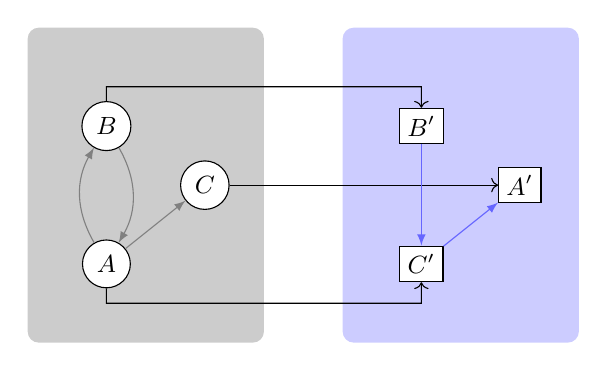
\begin{tikzpicture}
			\fill[rounded corners, gray!40] (0,0) rectangle (3,4);
			\fill[rounded corners, blue!20] (4,0) rectangle ++(3,4);
			%--
			\node[fill=white,inner sep=1mm,circle, draw, font=\small] (A) at (1,1) {\(A\)};
			\node[fill=white,inner sep=1mm,circle, draw, font=\small] (B) at (1,2.75) {\(B\)};
			\node[fill=white,inner sep=1mm,circle, draw, font=\small] (C) at (2.25,2) {\(C\)};
			\begin{scope}[xshift=4cm]
				\node[fill=white,inner sep=1mm, draw, font=\small] (A') at (1,1) {\(C'\)};
				\node[fill=white,inner sep=1mm, draw, font=\small] (B') at (1,2.75) {\(B'\)};
				\node[fill=white,inner sep=1mm, draw, font=\small] (C') at (2.25,2) {\(A'\)};
			\end{scope}
			\draw[->] (A) |- ++(4,-.5) -- (A');
			\draw[->] (B) |- ++ (4,.5) -- (B');
			\draw[->] (C) -- (C');
			%--
			\draw[-latex,gray] (A) -- (C);
			\draw[-latex,blue!60] (A') -- (C');
			\draw[-latex,gray] (A) to[bend left] (B);
			\draw[-latex,gray] (B) to[bend left] (A);
			\draw[-latex,blue!60] (B') -- (A');
		\end{tikzpicture}
	\end{center}
	\caption{\Todo{captione}}
\end{figure}
Le componenti \(A,B,C,\dots\) però ora non sono parte del discorso in un linguaggio naturale; sono `elementi' di una collezione --spesso gigantesca: \emph{tutti} i gruppi, \emph{tutte} le varietà differenziabili, senza eccezione-- \(\mathcal{L}\), che si chiamerà una `categoria'; Carnap definisce un funtore come una relazione funzionale tra linguaggi, che `preserva l'analisi logica'; per noi, un funtore è una relazione funzionale tra linguaggi, che preserva, in qualche modo da determinare, le relazioni che sussistono tra le loro diverse parti.

In questo senso la nozione data da Mac Lane ed Eilenberg in \cite{gtone} stava fondando un approccio \emph{relazionale}, dinamico, alla costruzione e alla comprensione degli oggetti matematici: le strutture non esistono di per loro, ma in una rete di relazioni, separate dalle quali esse sono incomprensibili, o comprensibili con maggiore fatica intellettuale.\footnote{H. Poincaré, il nonno della teoria delle categorie, disse che `la matematica non è solo un insieme di teoremi, così come una casa non è solo un mucchio di mattoni'. In maniera un po' più poetica (si veda il testo di Cook \cite{Cook1977-ry}) nella mitologia vedica, quando Indra immagina il mondo lo costruisce come una ragnatela o rete, in ciascuno dei cui nodi viene posto un gioiello; ogni \emph{dharma}, cioè ogni concetto sensibile o immaginabile, sia esso passato presente o futuro, è un nodo in questa rete, e la superficie di ciascun gioiello riflette ogni altro, cosicché ogni cosa che esiste implica tutte le altre (secondo il principio detto \emph{pratītyasamutpāda}, letteralmente traducibile come \emph{mutua produzione condizionata}).

	Questa nota non è il luogo adatta ad approfondire la questione dal punto di vista storico o filosofico (e ancor meno lo è questa introduzione); chi legge consulti \cite{marquis, kromer} per dei testi introduttivi sulla storia della teoria delle categorie --chi legge apprenderà lì che la teoria delle categorie ha molti precursori, che si possono far risalire molto più indietro nel tempo del 1945, anno della pubblicazione di \cite{gtone}. Un esempio su tutti, il cosiddetto \emph{programma di Erlangen} proposto da Klein in una famosa prolusione del 1872, \cite{Klein1893}.}

\medskip
Lo scopo di questa introduzione non è delineare una storia completa della teoria delle categorie; chi legge troverà nel libro di Kr\"omer \cite{kromer} un esempio già insuperabile, che è pienamente un testo \emph{di matematica}. La teoria delle categorie è ubiquitaria in ciò che la logica, l'algebra, la geometria moderna è stata dal secondo dopoguerra, tanto che è inestricabile dalla storia della matematica del ventesimo secolo, che è vasta e ancora in via di definizione; soprattutto, delineare questa storia non compete certamente a noi.

Il punto che vogliamo rendere esplicito qui ed ora è che fare quindi della teoria delle categorie una disciplina eminentemente astratta, che mal tollera motivazioni concrete dietro le definizioni --tali motivazioni sono sempre radicate nell'esperienza sensibile, solo talvolta un po' meno direttamente-- tradisce appieno la verità storica.

All'esatto contrario, lo spirito che ha animato la teoria delle categorie è quello di una comunità di matematici che hanno tentato indefessamente di spiegare in termini di pochi e semplici concetti essenziali la natura e il comportamento di costruzioni matematiche che a prima vista erano del tutto scorrelate tra loro: è stata edificata secondo scelte stilistiche che nella loro apparente ingenuità hanno dato diversi frutti. Senza nessuna pretesa di completezza o di autorità, proviamo a descrivere quali sono queste idee.
\begin{itemize}
	\item Gli assiomi che fondano una teoria devono essere pochi e ben motivati, vuoi dall'esperienza sensibile, vuoi dal numero elevato di esempi vantaggiosi che \emph{quegli} assiomi, e non altri, riescono a descrivere. Al di fuori della teoria delle categorie, la teoria della misura è un esempio relativamente buono di questo tipo di ragione.\footnote{Un famoso teorico delle categorie, J. Bénabou, produce un `cattivo esempio' che riportiamo senza pretesa di essere letterali (e soprattutto senza voler offendere nessuno): per costruire l'insieme delle coppie ordinate \((a,b)\) a partire da due insiemi \(A,B\) è necessario, formalmente parlando, considerare l'insieme \(2^{2^{A\cup B}}\), per poi restringere il discorso alle coppie di una certa forma ben precisa: la coppia ordinata \((a,b)\) consta dell'insieme \(\{\{a\},\{a,b\}\}\). In particolare, per considerare il prodotto cartesiano \(\mathbf{N} \times \mathbf{N}\) di due copie dei naturali (insieme di cui \emph{certamente} vogliamo essere in grado di parlare), va considerato l'insieme \(2^{2^{\mathbf{N} \cup \mathbf{N}}}\): insieme che è gigantesco, e Bénabou definisce `aberrante' la pratica di doverlo considerare per parlare di un oggetto tanto semplice quanto quello che contiene elementi tanto semplici quanto le coppie \((15,18), (3,7), (12, 259)\dots\)

		      In teoria delle categorie, invece, il prodotto cartesiano \(A\times B\) è definito in maniera molto più snella, e non meno rigorosa.}
	\item La matematica deve essere ispirata a un principio di ergonomia e modularità; deve essere relativamente semplice e intuitivo maneggiare gli enti che compongono una teoria, e deve essere chiaro come poter esportare alcuni suoi frammenti a un contesto diverso: che differenza c'è, in ultima istanza, tra un monoide, un anello, e un gruppo dove le operazioni di moltiplicazione e inversione sono continue rispetto a una topologia? In questo senso, la matematica deve essere ispirata a un canone simile a quello che orienta la scrittura di `buon' codice sorgente quando si programma. Tutti sono capaci di scrivere una funzione che calcola un fattoriale; già meno persone sono capaci di farlo tenendo d'occhio il costo computazionale, la leggibilità, la mantenibilità della teoria/libreria dove quel teorema/codice è immerso.
	\item Quando teorie diverse possiedono dei tratti comuni, esiste una spiegazione profonda, non accidentale, per questo. Lo scopo --o l'effetto-- di una parte piuttosto vasta di teoria delle categorie è stato di trovare questa spiegazione profonda, renderla evidente e cercare di portarla alle sue estreme conseguenze. Le applicazioni maggiori di questo principio si possono apprezzare in `discipline dalla natura altamente dialettica' (una locuzione rubata a \cite{lawvere1999profilo}, una lettura squisita che invitiamo chi legge a reperire ad ogni costo), come la geometria e la logica; ma abbondano anche gli esempi in algebra astratta (vedremo questa idea in azione proprio quando cercheremo di `spiegare' il motivo per cui tutti i teoremi di isomorfismo si somigliano tra loro).
	      % \item La matematica possiede un certo grado di auto-referenzialità: le teorie matematiche si possono apprezzare come un certo tipo particolare di oggetto matematico, che può essere compreso mediante il linguaggio matematico. Lungi dall'essere una fumosa affermazione filosofica, questa idea viene sostanziata mediante il linguaggio delle categorie.
\end{itemize}
L'opinione di noi che scriviamo è che questo punto di vista, al di là dei suoi meriti concreti, misurabili, confermi come lo scibile matematico sia alla portata di chiunque lo voglia cogliere, quando esso sia espresso in termini di pochi concetti fondamentali.

Quei concetti riusciranno poi a delineare cosa, all'interno delle verità del linguaggio, è una tautologia, e concentrare le proprie energie sul comprendere appieno ciò che non lo è. Se è vero che il discente paga un prezzo all'ingresso, perché non deve solo imparare definizioni e teoremi e tecniche di calcolo, ma soprattutto un modo di pensare diversamente (e ripensare, e ripensare ancora) a cosa è la matematica e al contempo \emph{disimparare} alcune abitudini, i rudimenti del linguaggio categoriale rendono più semplice, veloce ed efficiente apprezzare la natura intima di definizioni molto diverse tra loro, nate per risolvere problemi diversi, e sviluppate in dialetti diversi. 

Questo ha un costo cognitivo non indifferente: una indole poliedrica, e poco affine alla specializzazione, aiutano ad apprendere lo spirito dietro molte definizioni; ma questa indole, senza delle abilità di risolutore di problemi, rende impossibile \emph{fare i conti} adoperando le definizioni apprese.

\medskip
Lo scopo del libro che avete in mano è anche colmare questo abisso tra idee profonde, di ispirazione filosofica, generalista ed evocativa, e la natura eminentemente pratica (e quindi frustrante, pedissequa, quasi noiosa) del ragionamento matematico.

Ben più di una certa cattiva divulgazione, noi crediamo che questo approccio riesca a mostrare che la matematica è `alla portata di tutti', e secondo noi colpendo certamente più al cuore di alcuni tentativi.

\medskip
Esso nasce però anche con un fine molto più immediato: accompagnare un corso di teoria delle categorie che, durante l'anno accademico 2021-22 si è svolto online, su youtube, tenuto dal gruppo ItaCa (\url{https://progetto-itaca.github.io/pages/course.html}). Gli autori del libro sono i docenti di quel corso.

Ci ha spinto a impegnarci in questa ulteriore fatica il fatto che, con poche eccezioni, agli atenei italiani manca un corso il cui argomento principale sia la teoria delle categorie; solitamente si apprendono i suoi rudimenti perché è necessario introdurre delle costruzioni in geometria algebrica, algebra omologica, teoria degli anelli (e, sebbene molto raramente, in analisi).

Manca, invece, un corso che `riordini' le nozioni matematiche del discente unificandole sotto i pochi e fondamentali concetti della matematica strutturale. Questo è lo scopo concreto del libro che avete in mano.

\medskip
Come è strutturato, quindi, questo libro? E' innanzitutto suddiviso in capitoli, che rispecchiano la struttura del corso ma lo espandono laddove sia necessario (ad esempio, vi sono costruzioni ed esempi nel libro che non troverete a lezione; il capitolo \ref{cap:fattorizzazione} non è presente nel corso, eccetera); le sezioni di ogni capitolo si concludono con degli esercizi per il lettore, solitamente 3-5 per sezione. Gli esercizi sono risolti alla fine del libro, in una appendice; la ragione è che dopo i primi anni di studio della matematica, raramente si impiega un po' di tempo per mostrare agli studenti come si fanno gli esercizi, o per essere più precisi, quali sono le tecniche che il vecchio matematico, che le ha affinate con l'esperienza, sa essere valide per fare una dimostrazione. Non avere questo tipo di conferma della correttezza dei propri argomenti, o averlo solo dietro enorme insistenza, è molto castrante quando oltre a imparare definizioni, teoremi e corollari ci si trova a dover imparare un nuovo modo di ragionare.

Chi legge si accorgerà leggendo le soluzioni degli esercizi (ma dovrebbe farlo solo dopo aver provato a risolverli!) che esistono alcune tattiche di dimostrazione stabilite, che possono essere descritte in poche parole e che hanno un ampio campo di validità. Queste tecniche spesso si aiutano l'un l'altra.
\Todo{}
\medskip
Concludiamo questa introduzione parlando, finalmente, di matematica in senso stretto.

Lo scopo delle brevi sezioni che seguono e che chiudono il capitolo è di presentare quattro `preludi' categoriali, raccolti dai vari àmbiti del bagaglio culturale di uno studente che è alla fine di una laurea triennale in una generica università italiana.

L'accento, per ora, non è sul rigore, ma sul giusto grado di espressività e generalità.
\section*{Abelianizzazione, o `naturalità'}
Consideriamo un gruppo \(G\), la cui operazione è denotata moltiplicativamente; in esso, consideriamo il sottogruppo generato dagli elementi della forma
\[[x,y]:= xyx^{-1}y^{-1}\]
al variare di \(x,y\in G\). Si tratta quindi del sottogruppo i cui elementi sono i `commutatori' della forma
\[t = [x_1,y_1][x_2,y_2]\cdots[x_n,y_n]\]
al variare di \(x_i,y_i\in G\) e \(n\ge 0\) in \(\mathbf{N}\) (se \(n=0\), il prodotto è vuoto e quindi l'elemento in questione è uguale all'identità di \(G\)): è infatti facile vedere che l'inverso \([x,y]^{-1}\) di un commutatore è a sua volta un commutatore.

\`E altresì facile mostrare che il sottogruppo \([G,G]\) è normale in \(G\), e che è il sottogruppo minimale con la proprietà che il quoziente \(G/[G,G]\) è abeliano (cioè, se \(N\) è normale e \(G/N\) è abeliano, allora \(N\) contiene \([G,G]\)).

Il gruppo \(G/[G,G]\) prende il nome di \emph{abelianizzato} di \(G\), si denota a volte con \(G^\text{a}\), e soddisfa la seguente proprietà di \emph{universalità}:
\begin{quote}
	Esiste un unico omomorfismo \(\alpha : G \to G^\text{a}\) con la seguente `proprietà universale': per ogni omomorfismo di gruppi \(f : G \to A\), di codominio un gruppo abeliano \(A\), esiste un unico omomorfismo di gruppi \(\bar f : G^\text{a} \to A\) con la proprietà che \(\bar f \circ \alpha = f\).
\end{quote}
\begin{remark}
	Si può pensare a \(G\mapsto G^\text{a}\) come ad una `costruzione' che ad un gruppo \(G\) associa un altro gruppo \(G^\text{a}\), definito da una certa proprietà; questa associazione è poi responsiva al fatto che tra gruppi distinti \(G,H\) possono esistere degli omomorfismi \(f : G \to H\), nel senso che segue:
	\begin{quote}
		Dato un omomorfismo di gruppi \(f : G \to H\) esiste un omomorfismo \(f^\text{a} : G^\text{a} \to H^\text{a}\) tra gli abelianizzati di \(G,H\), definito mandando una classe di equivalenza \(g\cdot [G,G]\) in \(f(g)\cdot [H,H]\).
	\end{quote}
	L'unica cosa da verificare è che \(f^\text{a}\) così definita sia veramente una funzione; del resto, \(f\) discende al quoziente \(G^\text{a}\) partendo da una funzione \(\tilde f : G\to H^\text{a}\), cosa che segue immediatamente dal fatto che \(f\) manda \([G,G]\) in \([H,H]\) (perché \(f[x,y]=[fx, fy]\in [H,H]\)).
\end{remark}
Vi sono due proprietà che ora la corrispondenza \(f\mapsto f^\text{a}\) soddisfa: la loro verifica è a dir poco immediata.
\begin{enumtag}{fu}
	\item \label{fct_1} Se \(1_G\) è l'omomorfismo identico di un gruppo \(G\), allora \(1_G^\text{a}\) è l'omomorfismo identico di \(G^\text{a}\).
	\item \label{fct_2} Considerando due omomorfismi di gruppi componibili \(u : G\to H, v : H\to K\), si ha che
	\[(v\circ u)^\text{a} = v^\text{a} \circ u^\text{a}\]
	(l'uguaglianza di funzioni è una uguaglianza \emph{estensionale}, cioè valida elemento per elemento).
\end{enumtag}
Nelle stesse notazioni, si osservi anche che la definizione di \(f^\text{a} : G^\text{a} \to H^\text{a}\) è l'unica possibile qualora si chieda che \(f^\text{a}(\pi^G(x)) = \pi^H(f(x))\) per ogni \(x\in G\), ossia che il diagramma di omomorfismi
\[\xymatrix{
	G \ar[r]^-{\pi^G} \ar[d]_f & G^\text{a}\ar[d]^{f^\text{a}} \\
	H \ar[r]_-{\pi^H} & H^\text{a}
	}\]
sia commutativo.

La famiglia di omomorfismi \(\{\pi^G : G\to G^\text{a}\}\) è quindi specificata in maniera `uniforme' nel parametro da cui dipende, ossia è determinata, per un qualsiasi gruppo \(G\), dalla proiezione al quoziente \(\pi^G : G\to G/[G,G] : x\mapsto x\cdot[G,G]\) che manda un dato elemento nella sua classe laterale. In altre parole (meno precise, ma forse più evocative) per \emph{ogni} gruppo \(G\) è possibile costruire una funzione \(\pi^G : G\to G/[G,G]\), definita sempre alla stessa maniera in dipendenza di \(G\), in maniera tale che il quadrato precedente sia commutativo.

In situazioni simili, diciamo che l'assegnazione \(G\mapsto (\pi^G : G\to G^\text{a})\) è \emph{naturale}, o più precisamente che \(\pi^G\) è (la componente di) una \emph{trasformazione naturale}
\[\xymatrix{\boldsymbol\pi  : (\_) \ar@{=>}[r] & (\_)^\text{a}.}\]
Il dominio e il codominio di una trasformazione naturale sono dei \emph{funtori}: non daremo qui la definizione (che seguirà in \ref{sec_funtori}), ma l'idea che chi legge dovrebbe trattenere è che sappiamo trasformare un gruppo \(G\) in un altro gruppo \(F(G)\), e ogni omomorfismo di gruppi \(f : G\to H\) in un omomorfismo \(F(f) : F(G)\to F(H)\), in modo tale che le condizioni \ref{fct_1} e \ref{fct_2} siano verificate: quindi,
\begin{enumerate}
	\item Se \(1_G\) è l'omomorfismo identico, allora \(F(1_G)\) è l'omomorfismo identico di \(F(G)\).
	\item Considerando due omomorfismi componibili \(u : G\to H, v : H\to K\), si ha che
	      \[F(v\circ u) = Fv \circ Fu.\]
\end{enumerate}
In questo caso specifico, il dominio di \(\boldsymbol\pi\) è il funtore \emph{identico} definito in modo tautologico; il codominio è il funtore di abelianizzazione, la cui funtorialità è chiara grazie a \ref{fct_1} e \ref{fct_2}.
% \begin{remark}
% 	L'idea intuitiva che questa sezione vuole comunicare è che tutte le proprietà matematiche di una certa importanza si possono rifrasare nello stesso modo; la costruzione che produce \(G^\text{a}\) è un esempio particolare di una pratica generale, quella di definire un oggetto matematico mediante una certa \emph{proprietà universale}, che cioè somigli alla proprietà di \(G^\text{a}\).

% 	Siamo posti di fronte al problema di costruire un oggetto con certe proprietà. Se (è possibile trovarlo e) una volta che lo si è costruito esso soddisfa un requisito di universalità (che superficialmente cambia di volta in volta, ma che a conti fatti chiede sempre la stessa cosa: per ogni `diagramma' della tal forma, esiste un \emph{unico} omomorfismo della tale altra forma, per cui\dots), esso è \emph{univocamente determinato} da questa proprietà.
% \end{remark}
% \`E ora conveniente pensare agli omomorfismi di gruppo --e in effetti, relativi a qualsiasi altra struttura: i gruppi non hanno niente di speciale qui-- come `deformazioni' di una struttura di tipo \(G\) in una di tipo \(H\). In questo senso, l'assegnazione \(G\mapsto G^\text{a}\) è speciale in due sensi: prima di tutto, ogni gruppo \(G\) ha un omomorfismo canonico \(\pi_G : G \to G^\text{a}\) di proiezione al quoziente; secondo, per ogni \(f : G \to H\) le condizioni sopra sono verificate.
\section*{Teoremi di isomorfismo, o `universalità'}
I teoremi di isomorfismo nelle diverse strutture dicono tutti la stessa cosa
\section*{Completamenti, o `aggiunzioni'}
Dato uno spazio metrico \((X,d)\) una \emph{successione di Cauchy} è una successione \(a : \bbN \to X\) tale che per ogni \(\epsilon>0\) esiste un \(N\gg 1\) per cui
\[\forall n,m> N\; : \; d(a_n,a_m) < \epsilon.\]
Dato \((X,d)\) è sempre possibile costruire uno spazio metrico `completo' \(\bar X\) che contiene \(X\) come un sottospazio isometrico e tale che ogni successione \(a : \bbN \to \bar X\) che sia di Cauchy è convergente.

Questo spazio soddisfa la seguente proprietà: comunque sia dato uno spazio metrico completo \((Y,d_Y)\) e una mappa nonespansiva \(f : X\to Y\), esiste un'unico modo di estendere \(f\) a una mappa nonespansiva \(f^* : \bar X \to Y\) che coincide con \(f\) su \(X\le \bar X\).

Per costruire \(\bar X\), consideriamo lo spazio \((C^0(X,\bbR),d_\infty)\) delle funzioni continue \(X\to\bbR\), dotato della metrica unifome \((f,g)\mapsto \sup_x |fx-gx|\), che è facile mostrare è uno spazio metrico completo. Allora l'embedding \(j : X\mono \bar X\) è dato dalla funzione che manda \(x\) in \(\bar x = d(x,-) : X\to \bbR\), la quale è continua (e iniettiva, dato che la metrica è non degenere); dalla disuguaglianza triangolare segue che \(\sup_z|\bar{x}(z)-\bar{y}(z)|\le d(x,y)\) e in effetti vale l'uguaglianza, ponendo \(z=x\); ma allora, \(j : X\mono \bar X\) è una isometria.

Lo spazio così costruito
\section*{Il teorema di Brouwer, o `funtorialità'}
Dimostrare una cosa difficile `muovendo le mani'
\begin{exercises}
\item \label{ex_prelude_1} un exercise sul primo preludio
\item \label{ex_prelude_2} un exercise sul secondo preludio
\item \label{ex_prelude_3} Mostrare che \(j : X\to \bar X\) costruito in \autoref{} ha immagine densa; mostrare che \(\bar X\) è effettivamente tale che ogni successione di Cauchy converge; mostrare che il sottospazio \(j(X)\) è denso in \(\bar X\), ossia che ogni elemento \(f\) di \(\bar X\) è il limite \(\lim_n f_n\) di una successione di elementi della forma \(f_n=\bar x_n^f\)

Si riesce a costruire esplicitamente un'isometria \((\bbR, |\_|) \cong (C^0(\bbQ,\bbR), d_\infty)\)?
\item \label{ex_prelude_4} un exercise sul quarto preludio
\end{exercises}

\chapter{Categorie, funtori, trasformazioni naturali}

\section{Categorie}\label{categorie}

Prima di dare definizione formale di categoria, può essere di aiuto raccogliere degli esempi concreti per orientare i lettori.

La nozione di categoria, che introdurremo in \ref{def_categ}, riuscirà a unificare due strutture matematiche apparentemente molto diverse tra loro:
\index{Monoide}
\begin{definition}
	Un \emph{monoide} consiste in un insieme \(M\) dotato di
	\begin{itemize}
		\item un elemento \(e\in M\) (spesso denotato anche: $1_M$ o semplicemente $1$), chiamato \emph{elemento neutro}, \emph{unità} o \emph{identità} (si noti che da ciò segue, indirettamente ma immediatamente, che \(M\) è un insieme \emph{non vuoto}),
		\item Un'operazione binaria \(M\times M\to M\), detta \emph{prodotto} o \emph{composizione}, e indicata con \((m,n)\mapsto m\cdot n\) o con simili simboli infissi,
	\end{itemize}
	che soddisfano le seguenti proprietà:
	\begin{itemize}
		\item \emph{Unitalità}: per ogni \(m\in M\), i prodotti \(m \cdot e\) ed \(e\cdot m\) sono uguali a \(m\);
		\item \emph{Associatività}: per ogni \(m,n,p\in M\), i prodotti \((m\cdot n)\cdot p\) ed \(m\cdot (n\cdot p)\) sono uguali.
	\end{itemize}
\end{definition}
\index{Poset}
\begin{definition}
	% \Todo{poset}
	Un \emph{insieme preordinato} o \emph{preordine} o \emph{preset} consiste di un insieme \(P\) dotato di una operazione binaria \(\le\), solitamente indicata come un simbolo infisso \(x\le y\) per significare che \((x,y)\) è un elemento di \(\le\), che soddisfa le seguenti due proprietà:
	\begin{itemize}
		\item \emph{Riflessività}: per ogni $x\in P$, si ha $x\le x$;
		\item \emph{Transitività}: per ogni $x,y,z\in P$, si ha che
		\[(x\le y)\;\&\;(y\le z) \quad\implies\quad x\le z\]
	\end{itemize}
	Quando la relazione \(\le\) soddisfa anche la proprietà \emph{antisimmetrica}, cioè è tale per cui
		\[(x\le y)\;\&\;(y\le x) \quad\implies\quad x = y\]
	l'insieme \(P\), o meglio la coppia \((P,\le)\) si dice un insieme \emph{parzialmente ordinato} o \emph{poset}.
\end{definition}
Dimostreremo in \ref{mon_sonocat} e in \ref{pos_sonocat} rispettivamente che `ogni monoide è una categoria', e `ogni insieme preordinato (e a fortiori, ogni insieme parzialmente ordinato, dove la relazione \(\_\le\_\) è antisimmetrica) è una categoria'. (Gli enunciati in questione renderanno più precise queste affermazioni.)
\index{Categoria!--- degli insiemi finiti}
\begin{example}
	Un esempio naturale di categoria nasce considerando la classe \(\ctFin\) di tutti gli insiemi finiti \([n]\defeq \{1,\dots,n\}\) (con la convenzione che \([0]=\varnothing\) sia l'insieme vuoto), e le funzioni \(f : [n] \to [m]\) tra di loro. \`E evidente che non tutte tali funzioni sono componibili: una condizione necessaria --e sufficiente!-- affinché la composizione tra due funzioni \(f : [p] \to [q],g : [m] \to [n]\) tra insiemi finiti sia possibile è che il dominio dell'una coincida con il codominio dell'altra, ovvero che \(q=m\) e che le funzioni si possano `giustapporre' come
	\[\xymatrix{
			[p] \ar[r]^-f & [q] \ar[r]^-g & [r]
		}\]
	La composizione di funzioni \((f,g)\mapsto g\cmp f\) perciò è una operazione che ricorda quella di un monoide (per esempio, essa è associativa quando è definita) ma è \emph{parziale}, cioè non definita tra tutte le possibili coppie \((f,g)\) di funzioni tra insiemi finiti; quale che sia la struttura matematica che la classe degli insiemi finiti forma, perciò, essa non può essere un monoide. (Un altro motivo per cui \(\ctFin\) non può essere un monoide è che l'identità per la composizione di funzioni non è unica: \emph{ogni} insieme finito \([n]\) ha una sua propria funzione identica, e se \(f : [m]\to [n]\), si deve avere che \(f\cmp \id_{[m]}=f=\id_{[n]}\cmp f\) per funzioni identiche formalmente \emph{distinte}, sebbene definite `alla stessa maniera' da \(\lambda x.x : [n]\to [n]\) e \(\lambda y.y : [m]\to [m]\).)

	La classe \(\ctFin\) formerà una \emph{categoria}, e per lo stesso motivo faranno altrettanto
	\begin{itemize}
		\item \index{Categoria!---e di strutture algebriche} la classe \(\bbR\emdash\ctVect\) di tutti gli spazi vettoriali reali della forma \(\bbR^n\) per un \(n\ge 1\) naturale; non tutte le mappe lineari tra spazi vettoriali si possono comporre, e le applicazioni identiche sono tutte distinte;
		\item la classe di tutte le strutture algebriche di un dato tipo (gli insiemi, senza limite alla loro taglia; i gruppi, con gli omomorfismi di gruppo; gli spazi vettoriali, anche di dimensione infinita; gli spazi topologici, con le funzioni continue; eccetera).
	\end{itemize}
	% spazi vettoriali e mappe lineari tra di loro: gli spazi vettoriali \(\bbR^n\) per diversi \(n\), non tutte le mappe lineari si possono comporre. In particolare, una mappa \(f:\bbR^n\to \bbR^m\) si può comporre con una mappa \(g:\bbR^p\to\bbR^q\) solo se \(m=p\). In altre parole, \(g\) si può comporre con \(f\) solo se il codominio di \(f\) è uguale al dominio di \(g\).
	% Inoltre, non c'e solo una matrice identità, ma ce n'è una per ogni \(n\).
\end{example}
% La struttura algebrica che otteniamo è una \emph{categoria}, che definiamo a breve.
Una categoria sarà dunque, in prima approssimazione, una collezione di `entità' non meglio definite $A,B,X,Y,\dots$, legate tra loro da delle relazioni o `funzioni astratte' $f : X\to Y, g : A\to B$,\dots{} Questa intuizione è sufficiente per formulare la definizione di categoria, a cui deve però prima seguire una precisazione terminologica.

\index{Classe}
\index{Classe propria|see {Classe}}
Abbiamo utilizzato diverse volte la parola `classe': la definizione generale di categoria obbliga a farlo, dal momento che la collezione di tutte le strutture algebriche di un dato tipo è sempre `troppo grande per essere un insieme' (in un senso che formalizzeremo in dettaglio nell'Appendice \ref{fondamenti}); per il momento è sufficiente trattenere l'idea informale che una classe (o \emph{classe propria}) \(\ctC\) è una collezione di elementi che ha tutte le proprietà di un insieme, a parte quella di poter essere misurata da un numero cardinale.

Ogni volta che è necessario, useremo costruzioni elementari che si possono fare sulle classi come se esse fossero insiemi: per esempio se \(\ctA,\ctB\) sono classi, è lecito costruire la classe prodotto \(\ctA\times\ctB\), e considerare \emph{funzioni tra classi} \(F : \ctA\fun\ctB\), cioè sottoclassi \(F\) del prodotto \(\ctA\times\ctB\) che sono funzionali: per ogni elemento \(A\) della classe \(\ctA\), esiste un unico elemento \(B\in\ctB\) con \((A,B)\in F\), questo elemento si denota \(FA\), e a tutti gli effetti \(F\) si comporta come una funzione. Di nuovo, il linguaggio preciso che formalizza queste costruzioni verrà esposto nell'appendice \ref{fondamenti}; questa imprecisione iniziale sarà sempre del tutto innocua, e per il momento invitiamo chi legge a considerare il desiderio di approfondire la cosa solo una inutile distrazione.
\index{Categoria}
\begin{definition}[Categoria]\label{def_categ}
	Una \emph{categoria} \(\ctC\) consiste dei seguenti dati:
	\begin{enumtag}{c}
		\item\label{c_1} una classe \(\ctC_0\) i cui elementi chiamiamo \emph{oggetti}, di solito indicati con lettere latine maiuscole: \(A\), \(B\), \(X\), \(Y\),\dots
		\item\label{c_2} una classe \(\ctC_1\) i cui elementi chiamiamo \emph{morfismi} o \emph{frecce}, di solito indicati con lettere latine minuscole: \(f\), \(g\), \(h\),\dots
		\item\label{c_3} Ad ogni morfismo $f$ corrispondono due oggetti $\dom{f}$, $\cod{f}$ chiamati \emph{dominio} e \emph{codominio}. Per denotare il fatto che $f$ ha dominio $X\in\ctC_0$ e codominio $Y\in\ctC_0$, scriveremo $f\colon X\to Y$, o in \emph{forma diagrammatica}, $X \xrightarrow{f} Y$.
  \item\label{c_4} Ogni oggetto $X$ ha un morfismo distinto $\id_X\colon X\to X$ chiamato \emph{identità} o \emph{freccia identità}.
  \item\label{c_5} Per ogni coppia di morfismi $f\colon X\to Y$ e $g\colon Y\to Z$, cioè tali che $\cod{f}=\dom{g}$), è dato un morfismo $g\circ f:X\to Z$ chiamato \emph{composizione di $f$ e $g$}. Graficamente:
		\[
			\begin{tikzcd}
				X \ar{r}{f}
				\ar[rounded corners,out=-45, in=225]{rr}[swap]{g\cmp f}
				%    \ar[rounded corners,
				%             to path={ -- ([xshift=2ex]\tikztostart.south)
				%                       |- (T.center) \tikztonodes
				%                       -| ([xshift=-2ex]\tikztotarget.south)
				%                       -- (\tikztotarget)}]{rr}
				& Y \ar{r}{g} & Z \\
				&&
			\end{tikzcd}
		\]
		(Incidentalmente, osserviamo che \(\dom{g\cmp f}=\dom{f}\) e \(\cod{g\cmp f}=\cod{g}\).)
	\end{enumtag}
	A questi dati, chiediamo di soddisfare le seguenti proprietà:
	\begin{enumtag}{p}
		\item \label{p_1} \emph{Unitalità}: per ogni morfismo \(f:X\to Y\), le composizioni \(f\cmp\id_X\) e \(\id_Y\cmp f\) sono uguali ad \(f\).
		\item \label{p_2} \emph{Associatività}: dati oggetti \(X,Y,Z,W\) e morfismi \(f:X\to Y\), \(g:Y\to Z\) e \(h:Z\to W\), le composizioni \(h\cmp (g\cmp f)\) e \((h\cmp g)\cmp f\) sono uguali.
	\end{enumtag}
\end{definition}
\begin{notation}
	Dati due oggetti \(X\) e \(Y\), indichiamo con \(\Hom{\ctC}(X,Y)\) la classe di morfismi da \(X\) a \(Y\). Altre notazioni, come \(\mathrm{Hom}(X,Y)\) o \(\mathrm{Hom}_\ctC(X,Y)\), sono ugualmente comuni, e motivate dal fatto che le frecce di una categoria astraggono la nozione di \emph{omomorfismo} tra insiemi strutturati (si veda \ref{sigma_strutture} e l'esempio \ref{sigma_strutture_sono_cat}).
	% todo: mettere in una definizione sola "tutte" le categorie di strutture algebriche.
\end{notation}
\begin{remark}
	Si osservi che dalla definizione appena data discendono due corollari:
	\begin{itemize}
		\item Le classi \(\Hom{\ctC}(X,Y)\) al variare di \((X,Y)\in\ctC_0\times\ctC_0\) sono tutte disgiunte, perché la corrispondenza \(\ctC_1 \to \ctC_0\times\ctC_0\) che manda \(f\) nella coppia \(\dom{f},\cod{f}\) è una funzione (e allora la sua `fibra' sopra \((X,Y)\) è proprio \(\Hom{\ctC}(X,Y)\), disgiunto da \(\Hom{\ctC}(X',Y')\));
		\item come conseguenza immediata, se \(X\ne X'\) sono oggetti diversi, le identità \(\id_X,\id_{X'}\) sono morfismi diversi: si può cioè pensare la corrispondenza \(X\mapsto \id_X : \ctC_0\to\ctC_1\) come una funzione \emph{iniettiva} tra classi.
	\end{itemize}
\end{remark}
\begin{definition}[Categoria piccola, categoria localmente piccola]
	\index{Categoria!--- piccola}
	\index{Categoria!--- loc. piccola}
	Quando la classe \(\ctC_1\) è un insieme, come conseguenza dell'ultima osservazione fatta, è un insieme anche \(\ctC_0\): in tal caso chiamamo la categoria \(\ctC\) \emph{piccola}: le categorie \(\ctFin\) e \(\bbR\emdash\ctVect\) definite sopra sono piccole, perché abbiamo limitato enormemente la loro classe di oggetti: non abbiamo considerato \emph{tutti} gli insiemi finiti, ma solo quelli della forma \(\{1,\dots,n\}\).

	Invece, \(\ctC\) si dice \emph{localmente piccola} se dati ogni due oggetti \(X\) e \(Y\), la classe \(\Hom{\ctC}(X,Y)\) di morfismi da \(X\) a \(Y\) è un insieme. La categoria di \emph{tutti} gli insiemi finiti non è, strettamente parlando, piccola (perché c'è una classe propria anche solo di insiemi con un singolo elemento: \(\{\varnothing\},\{\{\varnothing\}\}, \{\{\{\varnothing\}\}\}\), eccetera), ma è localmente piccola, perché fissati due insiemi \(X,Y\), l'insieme delle funzioni \(f : X\to Y\) è un sottoinsieme di \(2^{X\times Y}\), e quest'ultimo è un insieme.
\end{definition}
\begin{remark}
	Gli assiomi di categoria non impediscono di costruire `categorie' dove \(\ctC_0\) è un insieme (per esempio, finito) e dove alcuni o tutti \(\Hom{\ctC}(X,Y)\) sono classi; queste costruzioni sono però relativamente innaturali, e non ne parleremo mai.
\end{remark}
Nel resto della sezione raccogliamo alcuni esempi classici di categorie, e nella successiva inizieremo a `costruire categorie nuove dalle vecchie', cioè a definire il \emph{prodotto} \(\ctC\times\ctD\) e la \emph{somma} \(\ctC+\ctD\) di due categorie date (si veda \ref{}), le categorie \emph{comma} \(\ctC/X\) e \emph{co-comma} \(X/\ctC\) sopra un oggetto \(X\in\ctC_0\) (si veda \ref{}), la categoria \emph{opposta} \(\ctC^\op\) di \(\ctC\), e molte altre.

La dicotomia essenziale che invitiamo il lettore ad apprezzare è questa:
\begin{itemize}
	\item le categorie sono strutture ideate per raccogliere una totalità di oggetti matematici di un dato tipo in una classe \(\ctC\) (in \emph{due} classi: gli oggetti e i morfismi) e studiarne le proprietà globali: le categorie (grandi) quindi sono `universi del discorso matematico'.
	\item D'altra parte le categorie sono anche delle strutture matematiche a sé stanti, modellate sulla nozione elementare di \emph{multigrafo diretto} (si veda \ref{}): le categorie (piccole) quindi sono esse stesse degli oggetti matematici che possiamo studiare alla stessa maniera di ogni altro oggetto matematico (e raccogliere in una loro totalità: ma questo discorso sarà approfondito solo molto più tardi, si veda \ref{}).
\end{itemize}
Si può imparare la teoria delle categorie in modo proficuo solo abbracciando \emph{entrambi} questi punti di vista, e ciò perché un dato ambito della matematica si occupa o `vive' in una (o più) categorie. Per esempio, l'algebra lineare studia le categorie \(\bbF\emdash\ctVect\) di spazi vettoriali, eventualmente su diversi campi di base. La topologia generale studia le categorie di spazi topologici, mentre la topologia differenziale si restringe alla categoria i cui oggetti sono varietà (e i morfismi funzioni differenziabili), oppure studia particolari categorie di strutture ordinate (perché l'insieme degli aperti di uno spazio topologico \(X\) con una topologia \(\tau \subseteq 2^X\) forma, con le operazioni di unione e intersezione, una struttura chiamata \emph{algebra di Heyting}, si veda \cite{}). Ma l'analisi funzionale studia quegli spazi \emph{vettoriali} (di dimensione infinita) che sono dotati di una \emph{topologia} metrizzabile (e determinata da un filtro di intorni dello zero), ed eventualmente di un prodotto scalare; la teoria della rappresentazione studia i \emph{gruppi} mediante omomorfismi in un gruppo di matrici, o le proprietà \emph{topologiche-differenziali} di questi gruppi di matrici (il gruppo ortogonale speciale, il gruppo dei quaternioni di norma 1, eccetera).

La seconda di queste osservazioni non è meno importante: porterà alla definizione di funtore (si veda \ref{def_funtore}), come \emph{omomorfismo tra categorie}, e alla definizione di trasformazione naturale (si veda \ref{sec_tnat}), come \emph{omomorfismo tra funtori}.

\medskip
Iniziamo ora a dare degli esempi di categorie piccole:
\index{Categoria!--- vuota}
\begin{example}
	La categoria vuota $\ctInit$ non ha oggetti né morfismi. Più formalmente, $\ctC_0,\ctC_1$ sono le classi vuote, e non è necessario specificare altra struttura per soddisfare (vacuamente) tutti gli assiomi di categoria.
\end{example}
\index{Categoria!--- terminale}
\begin{example}
La categoria terminale $\ctTerm$ ha un solo oggetto \(\bullet\), e un unico morfismo $\id_\bullet : \bullet\to\bullet$ che fa da identità. Chiaramente, non si può fare altro che porre $\id_\bullet\circ\id_\bullet=\id_\bullet$, e tutti gli assiomi di categoria sono soddisfatti.
\end{example}
\index{Categoria!--- discreta}
\`E sempre possibile dotare un insieme \(A\) della topologia discreta (o `massimale'), dove ogni sottoinsieme \(U\) di \(A\) è aperto, e della topologia indiscreta (o `minimale'), dove solo \(\varnothing\) e \(A\) sono aperti. Similmente, esistono due maniere, massimale e minimale, di considerare un insieme\footnote{Riguardo al problema se sia possibile dotare una classe propria della struttura di categoria discreta, la questione è apparentemente banale, ma in realtà tutt'altro che semplice da discutere: sebbene non ci sia alcun apparente problema ad assumere l'esistenza di classi proprie discrete, queste spesso vengono proibite assumendo un assioma a parte in aggiunta ai soliti della teoria degli insiemi/classi, detto \emph{principio di Vop\v enka}: un'idea intuitiva, ma leggermente imprecisa, di ciò che questo assioma afferma, è che nella classe propria di tutti gli insiemi non esiste una sotto-classe propria che sia discreta.} $A$ una categoria.
\begin{example}
	Dato un insieme $A$, la \emph{categoria discreta} su $A$, denotata $A^\delta$, ha per oggetti gli elementi $a\in A$, un unico morfismo identico $\id_a : a\to a$, e nessun altro. La composizione è forzata a essere definita solamente tra identità, nel modo più ovvio possibile, e tutti gli assiomi di categoria sono ovviamente soddisfatti.
\end{example}
\begin{example}
	Dato un insieme $A$, la \emph{categoria codiscreta} su $A$, denotata $A^\chi$ ha per oggetti gli elementi $a\in A$, e per ogni coppia di oggetti $a,a'\in A$, un unico morfismo $u_{aa'}:a\to a'$, e la composizione è definita da $u_{a'a''}\circ u_{aa'}=u_{aa''}$ (in particolare, da questo segue che esiste un unico elemento $\id_a=u_{aa}\in A^\chi(a,a)$).
\end{example}
Alcune categorie che è spesso utile considerare si rappresentano mediante dei grafi:
\index{Categoria!--- generica}
\begin{example}
	La categoria `freccia generica' ha due oggetti $0,1$ e un unico morfismo non identico $u : 0\to 1$ (che di solito non ha nome). La composizione è forzata a essere definita solamente tra le identità ed $u$, nell'unico modo ovvio, e tutti gli assiomi di categoria sono banalmente soddisfatti.
\end{example}
\begin{example}
	Più in generale, la categoria `catena di lunghezza $n+1$' è definita come segue:
	\begin{itemize}
		\item gli oggetti sono gli elementi di \(\{0,\dots,n\}\) (ci sono quindi $n+1$ oggetti, per ogni $n\ge 1$);\footnote{A volte è utile adottare la convenzione per cui quando $n=-1$, l'insieme $\{0,\dots,n\}$ è vuoto, e quindi la categoria `catena di lunghezza $0$' è la categoria vuota $\ctInit$ di \ref{}.}
		\item C'è un unico morfismo $i\to j$ se e solo se $i\le j$, di modo che esista un unico morfismo $i\to i$ (l'identità) per ogni $i\in\{0,\dots,n\}$, e un unico morfismo $i\to i+1$ per $i\in\{0,\dots,n-1\}$; in particolare l'unico morfismo $i\to j$ è ottenuto dalla composizione
		\[i\to i+1\to\dots\to j\]
	\end{itemize}
	\Todo{alcuni disegni}
\end{example}
\begin{example}
	\Todo{la `doppia freccia generica'}
\end{example}
\begin{example}
	\Todo{il quadrato generico, il cubo generico, l'\(n\)-cubo generico}
\end{example}
\begin{example}
	\Todo{lo `span generico' e il `cospan generico'}
\end{example}
\index{Categoria!--- libera}
Questi ultimi esempi lasciano supporre che \emph{ogni} grafo \(\ctG\), fatto di un insieme di vertici (o `oggetti') \(V\) e di un insieme di lati (o `morfismi') \(E\) generi una categoria \(F\ctG\). \`E effettivamente così, e la seguente costruzione in forma di esempio formalizza questa idea.
\index{Grafo}
\begin{example}
	Dato un grafo (o più propriamente, un \emph{multidigrafo}, ossia una coppia di insiemi \(E,V\) dotati di due funzioni \(s,t : E\rightrightarrows V\) che associano ad ogni \emph{lato} \(e\in E\) una coppia ordinata di \emph{vertici} \(se,te\in V\) detti il suo dominio o \emph{source} e il suo codominio o \emph{target}) \(\ctG\) possiamo definire la \emph{categoria libera} \(F\ctG\) su \(\ctG\) come segue:
	\begin{itemize}
		\item gli oggetti di \(F\ctG\) sono esattamente gli elementi di \(V\);
		\item i morfismi \(u\to v\) sono l'insieme
		      \[\sum_{n=0}^\infty E(u,x_1)\times\dots\times E(x_n,v)\]
		      di tutte le sequenze ordinate e finite di lati
		      \[ [\tup en;] : u \xto{e_1} x_1 \xto{e_2} x_2\xto{e_3} \dots\xto{e_{n-1}} x_{n-1}\xto{e_n} v\]
		      con la convenzione che se \(u=v\) ed \(n=0\) la sequenza vuota si interpreta come un laccio `banale' \([\;]_u : u\to u\), e usando la notazione, ovvia, \(E(x,y)\subseteq E\) per denotare i lati di source \(x\) e target \(y\).
	\end{itemize}
	La composizione di due sequenze \([\tup fm;]\) e \([\tup en;]\) è data dalla loro \emph{concatenazione}, ossia dalla operazione
	\[[\tup fm;]\circ[\tup en;] = [\tup fm;;\tup en;].\]
	Quando è definita, questa operazione è, evidentemente, associativa, e la sequenza vuota soddisfa la condizione di unitalità \ref{p_1} nella \ref{def_categ}.
\end{example}
Due esempi più elaborati, ma molto `concreti', di categorie dove gli oggetti sono numeri naturali:
\index{Categoria!--- dei circuiti}
\begin{example}
	\Todo{la categoria dei circuiti elettrici}
	La categoria $\cate{Circ}$ ha
	\begin{itemize}
		\item per oggetti i numeri naturali $0,1,2,\dots$;
		\item l'insieme dei morfismi $\cate{Circ}(m,n)$ consiste dell'insieme delle funzioni $\bbB^n\to \bbB^m$, dove $\bbB=\{0,1\}$ è l'insieme dei \emph{Booleani}\footnote{L'insieme $\bbB$ può essere interpretato come: l'insieme degli interi positivi modulo 2, l'insieme degli stati di un singolo bit di informazione; l'insieme \{sì, no\} delle risposte a una domanda; l'insieme $\{-1,1\}$ dei \emph{segni} assunti dagli elementi dell'immagine di una funzione reale, l'insieme \{acceso, spento\} degli stati di un interruttore, eccetera.} e $\bbB^0\defeq \{*\}, \bbB^{n+1}\defeq \bbB^n\times \bbB$ sono i prodotti cartesiani iterati di $\bbB$ con sé stesso.
	\end{itemize}
	Si noti che ogni funzione Booleana $f : \bbB^n\to\bbB^m$ risulta dal `prodotto' di $m$ funzioni Booleane \emph{semplici} $f_1,\dots,f_m : \bbB^n\to\bbB$, di modo che
	\[f(\tup xn,)=(f_1(\tup xn,),\dots,f_m(\tup xn,))\]
	Tra le funzioni Booleane semplici ci sono certamente le proiezioni canoniche $\pi_i : \bbB^n\to\bbB :(\tup xn,)\mapsto x_i$, ma anche le mappe diagonali $\Delta_m:\bbB\to\bbB^m$ definite da
	\[\Delta_m : x\mapsto (x,\dots,x)\quad m\text{ volte}\]
	Sull'insieme dei Booleani è possibile definire le operazioni logiche elementari di disgiunzione, congiunzione e negazione, che rappresentiamo graficamente con i seguenti diagrammi (noti a qualsiasi ingegnere elettronico)
	\[\begin{circuitikz}
		% \node[and port] (0,0) (myand1) {};
		\node[or port, fill=gray!10] (4,0) (or) {$\lor$};
		\node[xshift=3cm,and port, fill=gray!10] (0,0) (and) {$\land$};
		\node[xshift=5cm,not port, fill=gray!10] (0,0) (not) {$\lnot$};
		\node[font=\scriptsize] at (-1,-1) (z1) {$\_\lor\_ : \bbB^2\to\bbB$};
		\node[font=\scriptsize] at (2,-1) (z3) {$\_\land\_ : \bbB^2\to\bbB$};
		\node[font=\scriptsize] at (5,-1) (z2) {$\_\lnot : \bbB\to\bbB$};
	\end{circuitikz}\]
\end{example}
Vale il seguente teorema:
\begin{theorem}
	\Todo{qualcosa che dovrebbe essere nel libro di Walters \cite{Walters1992}, da cui ho preso questo esempio}
\end{theorem}
\index{Categoria!--- dei diagrammi di flusso}
\begin{example}
	\Todo{la categoria dei diagrammi di flusso}
\end{example}
Proseguiamo con degli esempi di categorie grandi:
\index{Categoria!--- degli insiemi}
\begin{example}
	\Todo{Insiemi finiti e funzioni (il primo esempio motivante)}
\end{example}
\index{Categoria!--- delle matrici}
\begin{example}
	\Todo{`Numeri naturali e matrici' (il secondo esempio motivante)}
\end{example}
\index{Categoria!--- degli insiemi}
\begin{example}
	\Todo{Tutti gli insiemi e funzioni, tutti gli spazi vettoriali}
\end{example}
\index{Categoria!--- degli ordinali}
\begin{example}
	\Todo{La categoria degli ordinali}
\end{example}
\index{Categoria!--- delle relazioni}
\begin{example}
	\Todo{Insiemi e relazioni}
\end{example}
\index{Categoria!--- di strutture algebriche}
\begin{example}
	\Todo{Gruppi/monoidi e omomorfismi}
\end{example}
\index{Categoria!---}
\begin{example}
	\Todo{Omomorfismi per una generica segnatura algebrica}
\end{example}
\index{Categoria!--- di spazi topologici}
\begin{example}
	\Todo{Spazi e funzioni continue}
\end{example}
\index{Categoria!--- di insiemi ordinati}
\begin{example}
	\Todo{Insiemi ordinati e funzioni monotone}
\end{example}
\index{Categoria!--- di funzioni parziali}
\begin{example}
	\Todo{Insiemi e funzioni parziali}
\end{example}
\index{Categoria!--- di insiemi puntati}
\begin{example}
	\Todo{Insiemi puntati}
\end{example}
\index{Categoria!--- di azioni di gruppo}
\begin{example}
	\Todo{Azioni di \(G\)}
\end{example}
\index{Categoria!--- di `stream'}
\begin{example}\label{example_streams}
	% \Todo{Streams (coalgebre per liste non vuote)}
	La categoria \(\cate{Stream}\) ha
	\begin{itemize}
		\item per oggetti gli insiemi \(A,B,C\dots\)
		\item per morfismi \(f : A\pto B\) le funzioni della forma
		      \[\longmor{f : \sum_{n=1}^\infty A^n}{B}\]
		      dove il dominio \(A^+=\sum_{n=1}^\infty A^n\) è l'insieme delle \emph{liste non vuote} di elementi di \(A\), cioè l'insieme \(A + (A\times A) + (A\times A\times A) + \dots\) i cui elementi sono sequenze ordinate della forma \((\tup an,)\) per \(n\ge 1\) e \(a_i\in A\) per ogni \(i=1,\dots,n\).\footnote{In termini più formali, \(A^+\) è il \emph{semigruppo libero} generato dall'insieme \(A\), un `semigruppo' essendo un insieme dotato di una operazione binaria associativa.}
	\end{itemize}
	L'intuizione dietro questa definizione è che un morfismo \(f \in \Hom{\cate{Stream}}(A,B)\) consiste di un `algoritmo' che data una lista non vuota di input \((\tup an,)\) calcola un output \(f(\tup an,)\in B\) (che chiaramente può dipendere anche da \(n\)), per ogni \(n\ge 1\).

	Le identità sono le funzioni \(\sum_{n=1} A^n\to A\) definite mandando \((\tup an,)\) in \(a_n\); la composizione è data, se \(f : A\pto B\) e \(g : B\pto C\) dalla regola \(g\circ f : A\pto C\)
	\[(\tup an,)\longmapsto g\big(f(a_1),f(a_1,a_2),\dots f(\tup a{n-1},),f(\tup an,)\big).\]
	Ovvero, la composizione \(g\circ f\) calcola l'output che la funzione \(g\) genera a partire dagli input \(f(a_1),f(a_1,a_2),\dots f(\tup a{n-1},),f(\tup an,)\).
\end{example}
% \begin{itemize}
%   \item Come accennato sopra, gli spazi vettoriali su \(\bbR\) e le mappe lineari formano una categoria, che chiamiamo \(\bbR\emdash\ctVect\). Più in generale possiamo definire la categoria \(\bbF\emdash\ctVect\), per un campo \(\ictF\), in maniera analoga.
%   \item Gli insiemi e le funzioni formano una categoria, che chiamiamo \(\ctSet\).
%   \item I gruppi e gli omomorfismi di gruppo formano la categoria \(\ctGrp\).
%   \item I gruppi abeliani e gli omomorfismi di gruppo formano la sottocategoria \(\ctAb\subseteq\ctGrp\). (Definiremo le sottocategorie a breve.)
%   \item Gli spazi topologici e le funzioni continue formano la categoria \(\ctTop\).
%  \end{itemize}
% \end{examples}
Veniamo ora a degli esempi più astratti e chiudiamo il cerchio su quelli che hanno motivato la definizione di categoria all'inizio.

Qualsiasi circostanza in cui una classe di strutture possiede una nozione ovvia di `omomorfismo' tale che
\begin{itemize}
	\item l'identità è un omomorfismo;
	\item la composizione di due omomorfismi è ancora un omomorfismo;
\end{itemize}
definisce la classe degli oggetti e dei morfismi di una categoria. (Gli esempi di strutture algebriche sono tutti di questo tipo; ne esistono altri, che non riguardano le operazioni algebriche: la composizione di due mappe proprie tra spazi di Hausdorff è ancora una mappa propria.)

Questo modo di intendere la definizione però oscura un'altra idea importante, perché potrebbe far sospettare che gli oggetti di una categori siano, alla fine, sempre insiemi dotati di strutture ulteriori (per esempio, operazioni o relazioni), e i morfismi funzioni che preservano queste strutture.

Invece, non tutte le categorie sono di questo tipo:
\Todo{qui sarebbe bello dire qualcosa di più, ma dobbiamo pensare a come}
\index{Relazione di equivalenza}
\begin{example}
	Un insieme dotato di una relazione di equivalenza si può vedere come una particolare categoria. Consideriamo un insieme \(X\) dotato di una relazione di equivalenza indicata con il simbolo \(\sim\).
	Definiamo la seguente categoria \(\ctB(X,\sim)\):
	\begin{itemize}
		\item Gli oggetti di \(\ctB(X,\sim)\) sono gli elementi di \(X\);
		\item Esiste un unico morfismo \(x\to y\) se e solo se \(x\sim y\) (e allora esiste anche un unico morfismo \(y\to x\)).
	\end{itemize}
	Per ogni oggetto \(x\), l'identità è l'unico morfismo \(x\to x\) dato dal fatto che la relazione è riflessiva (\(x\sim x\)).
	La composizione è data dalla transitività: se abbiamo morfismi \(x\to y\) e \(y\to z\) significa, in particolare, che \(x\sim y\) e \(y\sim z\). Per transitività, \(x\sim z\), e quindi c'è un unico morfismo \(x\to z\), che possiamo defiinre come composizione.

	Gli assiomi di unitalità e associatività sono automaticamente soddisfatti: per esempio, la composizione \((w\to x\to y)\to z\) e la composizione \(w\to (x\to y\to z)\) coincidono, constando dell'unico morfismo \(w\to z\).
\end{example}
Quello di \(\ctB(X,\sim)\) è un primo esempio di categoria in cui gli oggetti non sono insiemi con strutture ulteriori, ma non è quello minimale: la proprietà di \emph{simmetria} di \(\sim\) non serve per ottenere una categoria. Consideriamo i seguenti esempi (che raccogliamo in dei teoremi, di cui diamo una dimostrazione completa, perché questi esempi sono pedagogicamente rilevanti).
\index{Categoria!--- da una relazione}
\begin{theorem}\label{pos_sonocat}
	\Todo{ogni poset, e in effetti ogni preordine, definisce una categoria; copia da sotto}
\end{theorem}
\begin{theorem}
	\Todo{rovescio: una categoria dove ogni hom-set ha al piu un elemento è un preset}
\end{theorem}
\begin{examples}
	Una relazione d'ordine \((X,\le)\) si può vedere come una categoria, ancora una volta con un unico morfismo \(x\to y\) se e solo se \(x\le y\). Come nel caso delle relazioni di equivalenza, le identità sono date dalla proprietà riflessiva e la composizione dalla proprietà transitiva.

	Più in generale, un \emph{preordine} è una relazione riflessiva e transitiva, ma non necessariamente simmetrica o antisimmetrica. Ogni preordine si può vedere come una categoria.
\end{examples}
\index{Categoria!--- da un monoide}
\begin{theorem}\label{mon_sonocat}
	Un monoide si può vedere come una categoria con un solo oggetto --più precisamente, una categoria \emph{localmente piccola} con un solo oggetto.

	Dato un monoide \((M,\cdot,1)\), definiamo la seguente categoria, che indichiamo con \(\ctB M\).\footnote{A volte la categoria definita in questo modo si indica con \(\ctB(M,\cdot)\), a volte semplicemente con \(M\).}
	\begin{itemize}
		\item La categoria \(\ctB M\) ha un unico oggetto, che indichiamo con \(\star\);
		\item La categoria \(\ctB M\) ha un morfismo \(m:\star\to\star\) per ogni elemento \(m\in M\); l'unico hom-insieme che dobbiamo specificare, \(\Hom{\ctB(M,\cdot)}(\star,\star)\), è cioè uguale a \(M\), e in particolare, l'identità \(\id_\star\) è l'elemento neutro \(1\in M\);
		\item La composizione di morfismi
		      \[\longmor{\Hom{\ctB(M,\cdot)}(\star,\star)\times \Hom{\ctB(M,\cdot)}(\star,\star)}{\Hom{\ctB(M,\cdot)}(\star,\star)}\]
		      è data dal prodotto \(M\times M\to M\).
	\end{itemize}
\end{theorem}
Di converso,
\begin{theorem}
	\Todo{una categoria con un solo oggetto `è' un monoide}
\end{theorem}
\color{blue}
\begin{example}
	In un monoide, a differenza di una categoria generica, possiamo sempre comporre due morfismi \(m\) e \(n\): questo è garantito dal fatto che siccome c'è un solo oggetto, il dominio e il codominio di \(m\) ed \(n\) sono necessariamente uguali.

	Viceversa, data una categoria localmente piccola con un solo oggetto (indichiamolo ancora con questo simbolo, \(\bullet\)), l'insieme di morfismi \(\bullet\to\bullet\) ha una struttura di monoide con l'elemento neutro dato dall'identità, e il prodotto dato dalla composizione.

	L'unitalità e l'associatività del monoide e della categoria si corrispondono.
\end{example}

In particolare, ogni gruppo si può vedere come una categoria con un solo oggetto.
Dato un oggetto \(X\) di una categoria, un morfismo da \(X\) a \(X\) si chiama anche \emph{endomorfismo}. In un monoide, tutti i morfismi sono endomorfismi.

\begin{remark}
	Abbiamo visto che i gruppi sono gli oggetti della categoria \(\ctGrp\), ma anche che ogni gruppo si può a sua volta vedere come una categoria (con un solo oggetto). Entrambe le prospettive sono valide, e ce ne sono altre ancora.
	Allo stesso modo, gli ordini parziali sono categorie, ma si possono anche vedere come oggetti della categoria \(\ctPos\), dove i morfismi sono le funzioni monotone.
	Spesso, in teoria delle categorie, la stessa struttura matematica può apparire in modi diversi in contesti diversi, e questa varietà di prospettive è uno dei motivi per cui le categorie sono così versatili.
\end{remark}

% Concludiamo questa sezione con alcuni esempi estremi di categorie, utili per controesempi e casi limite.

% \begin{examples}
%  Consideriamo un insieme \(X\). Possiamo considerarlo una categoria in due modi:
%  \begin{itemize}
%   \item La \emph{categoria discreta su \(X\)} ha come oggetti gli elementi di \(X\), e gli unici morfismi sono le identità.
%   \item La \emph{categoria codiscreta su \(X\)} ha come oggetti gli elementi di \(X\), e un unico morfismo tra ogni due elementi.
%  \end{itemize}
%  La categoria discreta, equivalentemente, è la relazione di equivalenza discreta (la relazione di uguaglianza).
%  La categoria codiscreta si può vedere come un'unica grande classe di equivalenza su \(X\).
% \end{examples}

% \begin{example}
%  La \emph{categoria terminale} o \emph{unitaria}, che indichiamo con \(\cate{1}\), ha un solo oggetto e un solo morfismo (identità).
% \end{example}

% \begin{example}
%  La \emph{categoria vuota} non ha oggetti né morfismi.
% \end{example}

% Tutte le categorie descritte finora sono localmente piccole.


\subsubsection*{Esercizi}
\begin{enumerate}
	\item Un \emph{grafo diretto} (chiamato anche \emph{digrafo}) è un insieme \(V\), i cui elementi chiamiamo \emph{vertici}, e una relazione \(E\subseteq V\times V\), i cui elementi chiamiamo \emph{spigoli}. Diciamo che \(x\) è \emph{adiacente} a \(y\) se esiste uno spigolo \((x,y)\in E\). Un \emph{omomorfismo di grafi diretti} \(f:(V,E)\to (V',E')\) è una funzione \(f:V\to V'\) tale che se \(x\) è adiacente a \(y\), allora \(f(x)\) è adiacente a \(f(y)\). Dimostra che i grafi diretti e i loro omomorfismi formano una categoria.
	\item Un \emph{multigrafo diretto} (chiamato anche \emph{multidigrafo}) è definito similmente a un grafo diretto, ma può avere diversi spigoli tra gli stessi due vertici. Un multidigrafo consiste di un insieme \(V\) (i \emph{vertici}), e un insieme \(E\) (gli \emph{spigoli}), con due funzioni \(d_-,d_+:E\to V\), che associano un ``dominio'' e un ``codominio'' ad ogni spigolo. Un \emph{omomorfismo di multigrafi diretti} \((V,E)\to (V',E')\) consiste di una funzione \(f_0:V\to V'\) tra i vertici, e una funzione \(f_1:E\to E'\) tra gli spigoli, compatibili con le mappe \(d_-,d_+\) nel seguente modo:
	      \[
		      d_-(f_1(e)) = f_0(d_-(e)) ,\qquad d_+(f_1(e)) = f_0(d_+(e)) .
	      \]
	      Dimostra che \(f_1:E\to E'\) associa a uno spigolo tra \(x\) e \(y\) uno spigolo tra \(f_0(x)\) e \(f_0(y)\).
	\item Dimostra che i multigrafi diretti e i loro omomorfismi formano una categoria.
	\item Una categoria piccola si può vedere come un multigrafo con identità e composizione: riscrivi la definizione di categoria (piccola) in termini di multigrafi.  In che modo questa costruzione generalizza la definizione di monoide (come insieme con identità e composizione)?
	\item Un grafo diretto si può vedere come un multigrafo dove tra due vertici c'è al massimo uno spigolo. Dimostra che la costruzione al punto 3, se applicata ad un grafo diretto, dà un preordine.\Todo{Cambierei questo esercizio dato che preferirei dimostrare esplicitamente un enunciato analogo}
\end{enumerate}
\color{black}
\section{Isomorfismi}\label{isomorfismi}\index{Isomorfismo}
La nozione di isomorfismo tra due strutture di un dato tipo è certamente nota a chi legge, grazie ai primi corsi di algebra astratta.

Chi legge quindi ricorderà che quando due gruppi sono isomorfi, tutte le proprietà che si esprimono in termini degli assiomi di gruppo, e che sono godute dall'uno, sono godute anche dall'altro, e che grazie a ciò una strategia molto efficace per mostrare che due dati gruppi \emph{non possono} essere isomorfi è cercare una proprietà che sia goduta solo da uno dei due (per esempio, l'essere abeliano: ci sono certamente almeno due gruppi di ordine 24 distinti, il gruppo \emph{ciclico} \(\bbZ/24\bbZ\) e il gruppo \emph{simmetrico} delle permutazioni di 4 lettere \(\{a,b,c,d\}\)).
\Todo{Vorrei spiegare bene cosa significa: se \(G\iso H\), allora \(G\) è abeliano se e solo se lo è \(H\); del resto, \(7\in\bbZ/24\bbZ\iff 7\in\bbZ/12\bbZ\), che del primo è un sottogruppo proprio...}

La nozione di isomorfismo in teoria delle categorie generalizza molte di queste idee.
\begin{definition}[Isomorfismo]\label{def_isomorfismo}\index{Isomorfismo}\index{Morfismo!isomorfismo}
	Dati due oggetti \(X\) e \(Y\) in una categoria \(\ctC\), un \emph{isomorfismo} tra \(X\) e \(Y\) consiste di una coppia di morfismi \(f:X\to Y\) e \(g:Y\to X\) in direzioni opposte, tali che \(g\cmp f=\id_X\) e \(f\cmp g=\id_Y\).

	Il morfismo \(f\) è chiamato l'\emph{inverso} \(g^{-1}\) di \(g\) (e specularmente, \(g\) è l'inverso \(f^{-1}\) di \(f\)).

	Se esiste un isomorfismo tra \(X\) e \(Y\) diciamo che i due oggetti sono \emph{isomorfi} (spesso tralasciando mediante quale coppia di morfismi, dato che è chiaro dal contesto) e scriviamo \(X\iso Y\).\footnote{Formalmente parlando, \(X\iso Y\) è una quadrupla \((f,g, i,j)\) dove \(f : X\to Y, g: Y\to X\) e \(i,\) sono rispettivamente due dimostrazioni, che \(f\cmp g= \id_Y\) e che \(g\cmp f=\id_X\), però non insisteremo mai su questo dettaglio costruttivo.}
\end{definition}
\`E utile, sebbene del tutto ovvio, rappresentare mediante dei diagrammi commutativi il fatto che \(X,Y\) siano oggetti isomorfi: %un'interpretazione grafica: intuitivamente, un isomorfismo è una situazione dove l'applicazione di \(f\) si può invertire o annullare tramite \(g\), e viceversa, e si può sempre passare da \(X\) a \(Y\) senza perdere informazioni.
\[
	\begin{tikzcd}
		X\ar[d, "f"'] \ar[dr, equal, "\id_X"]& & Y \ar[dr, equal, "\id_Y"]\ar[d,"g"']\\
		Y \ar[r, "g"']& X & X \ar[r, "f"']& Y
	\end{tikzcd}
\]
Normalmente si indica la coppia \((f,g)\) solo con \(f\) o con \(g\), lasciando l'inverso implicito (tale inverso, se esiste, è unico, si vedano gli esercizi, e ciò ci autorizza a usare il singolare nella definizione).
\begin{examples}
	Raccogliamo degli esempi di isomorfismo in varie categorie:%La definizione di isomorfismo comprende molte delle nozioni di ``struttura equivalente'' usate in matematica:
	\begin{enumtag}{ei}
		\item \`E evidente che in ogni categoria \(\ctC\), tutte le identità \(\id_X : X\to X\) sono isomorfismi che coincidono col loro inverso, e che la composizione di isomorfismi $f_1\circ f_2$ è un isomorfismo di inverso $g_2\circ g_1$, cioè (come è noto a chiunque abbia sostenuto con profitto un esame di teoria dei gruppi) $(f_1\circ f_2)^{-1} = f_2^{-1}\circ f_1^{-1}$.
		\item In \(\ctSet\), gli isomorfismi sono esattamente le biiezioni, o `corrispondenze biunivoche'. Per la definizione solitamente data di cardinalità, due insiemi sono isomorfi se e solo se hanno lo stesso numero cardinale, che quindi risulta essere una scelta privilegiata di un elemento isomorfo a un dato insieme.
		\item In \(\bbR\emdash\ctVect\), gli isomorfismi sono le biiezioni lineari. In particolare, due spazi vettoriali $V,W$ di dimensione finita $\dim V=n,\dim W=m$ sono isomorfi se e solo se $n=m$.
		\item In \(\ctTop\), gli isomorfismi sono gli \emph{omeomorfismi}: funzioni continue con un'inversa insiemistica anch'essa continua. Si noti come questo mostra che può non accadere che, se \(f : X\to Y\) è un omomorfismo biiettivo, la \emph{funzione} inversa \(g : Y\to X\) sia anch'essa un isomorfismo; per esempio, l'identità \(\id_X : (X,\delta)\to (X,\gamma)\) su un insieme con tre punti \(X=\{a,b,c\}\) è continua quando \(\delta\) è la topologia discreta e \(\gamma\) è la topologia banale, ma la sua inversa insiemistica \(\id_X : (X,\gamma)\to(X,\delta)\) \emph{non} è continua.
		\item In ogni categoria di strutture algebriche (si veda \ref{}), gli isomorfismi sono gli isomorfismi di \(\Sigma\)-strutture, cioè le funzioni \(f : A\to B\) che sono \(\Sigma\)-omomorfismi biiettivi, la cui inversa insiemistica è ancora un \(\Sigma\)-omomorfismo.
	\end{enumtag}
\end{examples}
\begin{warning}
	Spesso una categoria viene chiamata con il nome dei suoi oggetti (\(\ctVect\), \(\ctGrp\), eccetera), ma per decidere se due oggetti sono isomorfi è essenziale sapere \emph{quali sono i morfismi} per sapere che struttura in particolare vogliamo preservare. Per esempio, tutte le potenze \(\bbR,\bbR^2,\bbR^3,\dots\) sono isomorfe come insiemi (hanno la stessa cardinalità \(2^{\aleph_0}\)); ma non come spazi vettoriali reali (hanno dimensioni diverse) né come varietà differenziabili (hanno dimensioni diverse; ma il teorema di invarianza della dimensione per varietà non è completamente ovvio), ma lo sono come gruppi abeliani (o come spazi vettoriali \emph{sui razionali}, il che è leggermente controintuitivo: infatti la dimostrazione dipende dall'assioma della scelta).

	Per cui, nella categoria \(\ctSet\), gli oggetti \(\bbR\) e \(\bbR^2\) sono isomorfi, ma non sono isomorfi se li intendiamo come oggetti della categoria \(\bbR\emdash\ctVect\), e lo sono invece in \(\bbQ\emdash\ctVect\).
\end{warning}
% Si noti che le condizioni \(g\cmp f = \id_X\) e \(f\cmp g=\id_Y\) servono entrambe, perché possono valere o non valere indipendentemente l'una dall'altra.
% \begin{example}
%  Nella categoria \(\bbR\emdash\ctVect\), si consideri la mappa \(f:\bbR\to\bbR^2\) data dall'inclusione dell'asse \(X\), \(x\mapsto(x,0)\). Data la proiezione sull'asse \(X\) data da \(g:\bbR^2\to\bbR\), \((x,y)\mapsto x\), si ha che \(g\cmp f=\id_\bbR\). Però non è vero che \(f\cmp g = \id_{\bbR^2}\). (E infatti i due oggetti non sono isomorfi come spazi vettoriali.)
% \end{example}

\begin{definition}[Gruppoide]\label{def_gruppoide}\index{Categoria!Gruppoide}
	Una categoria in cui tutti i morfismi sono isomorfismi si chiama \emph{gruppoide}.\footnote{In inglese \emph{groupoid}. Da notare che una vecchissima terminologia coniata dal matematico norvegese Øystein Ore chiama `gruppoidi' quelli che oggi sono detti \emph{magmi}, insiemi dotati di una operazione binaria --e nessun altro assioma. Noi non useremo mai la terminologia di Ore.}
\end{definition}
\begin{example}[\(\ctB(X,\sim)\) come gruppoide]\label{exa_releq_groupoid}
	Abbiamo visto che un preordine (una relazione riflessiva e transitiva) si può vedere come una categoria. Questa categoria è un gruppoide se e solo se la relazione è anche simmetrica (cioè, è un'equivalenza). Se \(x\sim y\), abbiamo un unico morfismo \(x\to y\). Questo morfismo è invertibile se e solo se esiste un morfismo \(y\to x\), cioè, se anche \(y\sim x\). (Si noti che non ci sono altre condizioni da soddisfare per avere un inverso: per esempio, il morfismo composto \(x\to y\to x\) è necessariamente uguale a \(\id_x\) per unicità.)
\end{example}
\begin{example}[\(\ctB(G,\cdot,1)\) come gruppoide]\label{exa_grp_groupoid}
	Abbiamo visto che ogni monoide \(M\) si può considerare una categoria con un solo oggetto. Questa categoria è un gruppoide se e solo se \(M\) è un gruppo. Infatti, un morfismo \(m\) ammette un inverso nel senso della teoria delle categorie se e solo se ammette un inverso nel senso della teoria dei gruppi: \(g\cdot g^{-1}=g^{-1}\cdot g = e\).
\end{example}

Un \emph{automorfismo} è un endomorfismo (un morfismo da un oggetto a sé stesso) invertibile. In un gruppo, tutti i morfismi sono automorfismi.

\begin{example}
	La categoria i cui oggetti sono gli insiemi e i cui morfismi sono biiezioni è un gruppoide. Quando si prendono solo gli insiemi finiti, questa categoria diventa molto interessante: consta della `unione disgiunta' (in un senso che preciseremo in \ref{}) di tutti i gruppi simmetrici\Todo{}
\end{example}

L'esempio precedente si può vedere come una sottocategoria di \(\ctSet\).
Più in generale, in virtù del fatto che ogni identità \(\id_X\) è un isomorfismo, e del fatto che la composizione di isomorfismi è un isomorfismo, data una categoria \(\ctC\) possiamo sempre prendere la sottocategoria che contiene tutti gli oggetti e tutti i suoi isomorfismi.
\begin{definition}
	Il \emph{cuore} di una categoria \(\ctC\) è il gruppoide ottenuto prendendo
	\begin{itemize}
		\item come oggetti gli oggetti di \(\ctC\),
		\item come morfismi \(X\to Y\) gli isomorfismi di \(\ctC\) da \(X\) a \(Y\).
	\end{itemize}
\end{definition}

Si vedano gli esercizi sul perché in questo modo si ottenga una categoria (con identità e composizione).

\begin{definition}[Categoria scheletrica]\label{def_cat_scheletrica}\index{Categoria!--- scheletrica}
	Una categoria \(\ctC\) si dice \emph{scheletrica} se vale la seguente proprietà:
	\[X\iso Y \, (\text{mediante } f,g) \,\Rightarrow\, (X=Y \,\&\, f=g=\id_X),\]
	cioè se gli unici isomorfismi che esistono tra due oggetti sono le identità (si veda \ref{}).
\end{definition}
\subsubsection*{Esercizi}
\begin{enumerate}
	\item Mostrare che la composizione nella categoria \(\cate{Stream}\) definita in \ref{example_streams} è effettivamente associativa, e l'assioma di identità è effettivamente valido. %Dato un morfismo \(f:X\to Y\) in una categoria \(\ctC\), dimostra che se un inverso per \(f\) esiste, allora è unico.
	\item Caratterizzare gli isomorfismi nelle seguenti categorie: \Todo{lista}
	\item Dati due spazi metrici \((X,d)\) e \((Y,d')\), ricorda che una funzione \(f:X\to Y\) si dice \emph{Lipschitz continua} se soddisfa la disuguaglianza
	      \[
		      d'(fx,fx')\le \alpha d(x,x')
	      \]
	      per ogni \(x,x'\in X\) e per qualche \(\alpha\in\bbR_{>0}\); in tal caso, l'inf di tutti questi \(\alpha\) si chiama la \emph{costante di Lipschitz} di \(f\); dimostrare che gli spazi metrici e le funzioni Lipschitz continua sono oggetti e morfismi di una categoria, chiamata \(\cate{MetLip}\); caratterizzre gli isomorfismi di \(\cate{MetLip}\). Fornire un esempio di due spazi metrici isomorfi in \(\ctTop\), ma non in \(\cate{MetLip}\).

	      Ripetere tutte queste domande rispetto alla definizione, più generale, di funzioni \emph{\(K\emdash\alpha\)-h\"olderiane} tra spazi metrici, ricordando che una funzione \(f : (X,d)\to (Y,d')\) si dice \(K\emdash\alpha\)-h\"olderiana quando
	      \[d'(fx,fx')\le Kd(x,x')^\alpha\]
	      per \(K\in \bbR_{\ge 0}\) e \(\alpha\in \bbR_{>0}\).
	\item Costruisci un esempio in \(\ctTop\) di oggetti \(X\) e \(Y\) non isomorfi, e morfismi \(f:X\to Y\) e \(g:Y\to X\) tali che \(g\cmp f=\id_X\) (ma \(f\cmp g \ne \id_Y\)).
	      % \item Dimostra che in ogni categoria, le identità sono isomorfismi, e che la composizione di isomorfismi è un isomorfismo.
	      %       \Todo{Trovo questi esercizi un po' troppo facili\dots Non che sia un male, ma vorrei degli esempi più pedagogici!}
	\item In una categoria localmente piccola \(\ctC\), dati due oggetti isomorfi \(X\) e \(Y\), dimostra che per ogni oggetto \(A\), gli insiemi \(\Hom{\ctC}(A,X)\) e \(\Hom{\ctC}(A,Y)\) sono in corrispondenza biunivoca.
\end{enumerate}
\section{Operazioni tra categorie}

\Todo{categoria prodotto, categoria somma, categoria opposta,}
\Todo{categorie slice e coslice}
\Todo{spazi puntati come coslice}
\Todo{scheletro di una categoria}
\Todo{categoria dei morfismi}
\Todo{Categoria degli `span' e dei `cospan'}

\section{Funtori e diagrammi}

\Todo{motivazione: se i monoidi e i poset sono categorie, a che tipo di trasformazione tra categorie corrispondono gli omomorfismi di monoide e le funzioni monotone? Ottima domanda!}
\begin{definition}[Funtore]\label{def_funtore}\index{Funtore}
	Date due categorie \(\ctC\) e \(\ctD\), un \emph{funtore} \(F:\ctC\fun\ctD\) consiste dei seguenti dati.
	\begin{itemize}
		\item Un'assegnazione ad ogni oggetto \(X\) di \(\ctC\) di un oggetto \(FX\) di \(\ctD\);
		\item Un'assegnazione ad ogni morfismo \(X \xrightarrow{f} Y\) di \(\ctC\) di un morfismo \(FX \xrightarrow{Ff} FY\) di \(\ctD\) (si noti che \(F(\dom{f})=\dom{Ff}\) e \(F(\cod{f})=\cod{Ff}\));

		      che soddifa le seguenti proprietà.
		\item \emph{Preservazione delle identità}: per ogni oggetto \(X\) di \(\ctC\), \(F(\id_X)=\id_{FX}\);
		\item \emph{Preservazione delle composizioni}: per ogni coppia di morfismi componibili \(f\) e \(g\) di \(\ctC\), \(F(g\cmp f)=Fg\cmp Ff\).
	\end{itemize}
\end{definition}

% esempi: funzioni monotone
% esempi: omomorfismi
% esempi: rappresentazioni e azioni di gruppo
% funtori controvarianti, prefasci, bifuntori
% hom come funtore
% esempi: funtori ``dimenticanti''
% esempi: funtori ``liberi''
% C -> Sk(C) "è un'equivalenza"
% altri esempi?
% composizione di funtori, la (1-)categoria Cat

% diagrammi
% diagrammi commutativi (voglio una definizione precisa)
% funtori li preservano - in particolare, preservano iso

\subsubsection*{Esercizi}
\begin{enumerate}
	\item
	\item
	\item
	\item
	\item
\end{enumerate}

\subsubsection*{Esercizi}
\begin{enumerate}
	\item
	\item
	\item
	\item
	\item
\end{enumerate}


\section{Trasformazioni naturali}\label{sec_tnat}

\subsubsection*{Esercizi}
\begin{enumerate}
	\item
	\item
	\item
	\item
	\item
\end{enumerate}

\section{Monomorfismi ed epimorfismi}


Siccome i monoidi corrispondono precisamente alle categorie con un solo oggetto, come visto nell'esempio \ref{mon_sonocat},
la definizione di elemento di un monoide cancellabile a sinistra o a destra si può applicare direttamente ai morfismi delle categorie da loro indotte.
Ricordiamo che un elemento \(x\) di un monoide \((M, \cdot, 1)\) si dice cancellabile a sinistra (rispettivamente, destra) se,
per ogni coppia di elementi \(y_0\) e \(y_1\) in \(M\) tali che \(x \cdot y_0 = x \cdot y_1\) (rispettivamente, \(y_0 \cdot x = y_1 \cdot x\)),
si ha che \(y_0 = y_1\).

Se però vogliamo estendere tale definizione ad una categoria generica,
la cui composizione è dunque un'operazione parziale,
è necessario considerare solo le composizioni ben definite
(ovvero tra frecce consecutive).
Si arriva così alle seguenti definizioni.

\begin{definition}[Monomorfismo]\label{def_Mono}\index{Monomorfismo}\index{Morfismo!mono---}
	Un morfismo \(m \colon B \to X\) in una categoria \(\ctC\) è un \emph{monomorfismo} (o \emph{mono}) se,
	per ogni coppia di frecce parallele \(f, g \colon A \to B\) in \(\ctC\) tali che \(m \cmp f = m \cmp g\), si ha che \(f = g\).
	%Equivalentemente, \(m\) è un monomorfismo se è cancellabile a sinistra, ovvero \(m \cmp f = m \cmp g\) implica \(f = g\) ogni qual volta la scrittura ha senso (ovvero quando \(f\) e \(g\) sono frecce parallele e pre-componibili con \(m\)).
\end{definition}

\begin{definition}[Epimorfismo]\label{def_Epi}\index{Epimorfismo}\index{Morfismo!epi---}
	Un morfismo \(e \colon X \to A\) in una categoria \(\ctC\) è un \emph{epimorfismo} (o \emph{epi}) se,
	per ogni coppia di frecce parallele \(f, g \colon A \to B\) in \(\ctC\) tali che \(f \cmp e = g \cmp e\), si ha che \(f = g\).
	%Equivalentemente, \(e\) è un epimorfismo se è cancellabile a destra, ovvero \(f \cmp e = g \cmp e\) implica \(f = g\) ogni qual volta la scrittura ha senso (ovvero quando \(f\) e \(g\) sono frecce parallele e post-componibili con \(e\)).
\end{definition}

Siccome le definizioni categoriali di mono ed epi generalizzano, rispettivamente, quelle, algebriche, di elementi cancellabili a sinistra e a destra,
otteniamo immediatamente il seguente esempio.

\begin{example}
	Nella categoria indotta da un monoide, i mono sono gli elementi cancellabili a sinistra,
	e gli epi sono gli elementi cancellabili a destra.
\end{example}

Vediamo ora invece esempi in categorie non indotte da monoidi.
Il primo caso, alquanto degenere, è dato dai preordini. 

\begin{example}
	Nella categoria indotta da un preordine, come visto nell'esempio~\ref{???},
	tutti i morfismi sono sia epi che mono.
	Infatti, la definizione di epi e mono è sempre soddisfatta banalmente,
	dato che, in un preordine, due frecce parallele sono necessariamente uguali.
\end{example}

Gli esempi precedenti mostrano come
un morfismo possa essere sia epi che mono, e comunque non essere un isomorfismo.
Il prossimo esempio, rispetto ai precedenti, è più complesso.

% TODO: Lo svolgimento dell'esempio dovrebbe invece essere un esercizio svolto? Come lo formattiamo?
\begin{example}
	In \(\ctSet\), la categoria degli insiemi, i monomorfismi sono precisamente le funzioni iniettive
	e gli epimorfismi sono precisamente le funzioni surgettive.

	Consideriamo il caso delle funzioni surgettive.
	Se \(e \colon X \to A\) è una funzione surgettiva e \(f, g \colon A \to B\) sono funzioni tali che \(f \cmp e = g \cmp e\),
	allora per ogni elemento \(a \in A\) esiste un \(x \in X\) tale che \(e(x) = a\), per la surgettività di \(e\).
	Osserviamo che \((f \cmp e)(x) = (g \cmp e)(x)\), ovvero \(f(e(x)) = g(e(x))\),
	ma allora \(f(a) = g(a)\).
	Per la genericità di \(a\) concludiamo che \(f = g\), e dunque \(e\) è epi.

	Nel caso opposto, in cui \(e \colon X \to A\) è epi, sia \(a \in A\).
	Assumiamo per assurdo che non esista \(x \in X\) tale che \(f(x) = a\).
	Allora siano \(k_0 \colon A \to \{0, 1\}\) la funzione costante in \(0\),
	e \(\delta_a \colon A \to \{0, 1\}\) la funzione caratteristica di \(a\) in \(A\).
	Siccome \(a\) non appartiene all'immagine di \(e\), abbiamo che \(k_0 \cmp e = \delta_a \cmp e\)
	in quanto entrambe le composizioni assumono costantemente il valore \(0\) su tutto il dominio \(X\).
	Dunque, \(k_0 = \delta_a\), il che è assurdo.
	Dalla negazione dell'ipotesi per assurdo, concludiamo che \(e\) è surgettiva.
\end{example}

Si noti che la dimostrazione che le funzioni surgettive sono epi sarebbe immediata
se usassimo il fatto che ogni funzione surgettiva ha un'inversa destra.
L'esistenza dell'inversa destra, però, è una conseguenza dell'assioma di scelta,
che invece non viene impiegato nella dimostrazione di cui sopra.

\begin{exercise}
	Dimostrare che una funzione è iniettiva se e solo se è un mono in \(\ctSet\),
	ma senza utilizzare il fatto che le funzioni iniettive hanno inversa sinistra.
\end{exercise}

Per ragioni che saranno evidenti nella prossima sezione,
abbiamo evidenziato come l'equivalenza tra funzioni surgettive (iniettive)
e epi (mono) in \(\ctSet\) sia indipendente dall'esistenza di un'inversa destra (sinistra).

\begin{remark}
\label{rmk:mono-epi-duality}
Le nozioni di monomorfismo ed epimorfismo sono duali:
un morfismo in una categoria \(\ctC\) è mono (epi) se e solo se è epi (mono) in \(\ctC^{\op}\) (vedi \ref{???}).
\end{remark}

Dimostriamo ora alcuni risultati che rendono più agevole lavorare con mono ed epi,
sfruttando la dualità a nostro vantaggio.

\begin{proposition}
	Siano \(f \colon A \to B\) e \(g \colon B \to C\) due frecce consecutive in una qualche categoria.
	Allora:
	\begin{enumerate}
		\item Se \(f\) e \(g\) sono entrambe mono (epi), allora anche \(g \cmp f\) è mono (epi).
		\item Se \(g \cmp f\) è mono, allora anche \(f\) è mono.
		\item Se \(g \cmp f\) è epi, allora anche \(g\) è epi.
	\end{enumerate}
\end{proposition}
\begin{proof}
	Grazie all'osservazione~\ref{rmk:mono-epi-duality},
	ci basta dimostrare il risultato per i mono,
	e il risultato per gli epi segue per dualità.
	\begin{enumerate}
		\item Siano \(f\) e \(g\) mono.
		Per dimostrare che \(g \cmp f\) è mono,
		consideriamo una coppia di frecce parallele \(h\) e \(k\) tali che \((g \cmp f) \cmp h = (g \cmp f) \cmp k\).
		Per associatività della composizione, \(g \cmp (f \cmp h) = g \cmp (f \cmp k)\).
		Allora, siccome \(g\) per ipotesi è mono, si ha che \(f \cmp h = f \cmp k\).
		Inoltre, siccome \(f\) per ipotesi è mono, si ha che \(h = k\).
		Quindi, per la generalità di \(h\) e \(k\), si ha che anche \(g \cmp f\) è mono.
		\item Assumiamo che \(g \cmp f\) sia mono.
		Per dimostrare che \(f\) è mono,
		consideriamo una coppia di frecce parallele \(h\) e \(k\) tali che \(f \cmp h = f \cmp h\).
		Allora, post-componendo con \(g\) su ambo i lati e sfruttando la associatività della composizione,
		otteniamo che \((g \cmp f) \cmp h = (g \cmp f) \cmp k\).
		Siccome per ipotesi \(g \cmp f\) è mono, si ha che \(h = k\).
		Quindi, per la generalità di \(h\) e \(k\), si ha che anche \(f\) è mono. \qedhere
	\end{enumerate}
\end{proof}

\begin{proposition}[Una proprietà di mono ed epi in \(\ctSet\)]
	Dato un quadrato commutativo di funzioni
	\[\begin{tikzcd}
			E \ar[r,"f"]\ar[d, "e"']& A\ar[d, "m"] \\
			B \ar[r, "g"']\ar[ur,dashed,"u"] & X
		\end{tikzcd}\]
	dove \(e : E\to B\) è un epi e \(m : A \to X\) un mono, esiste un unica funzione \(u : B\to A\) (indicata con una freccia tratteggiata) con la proprietà di `spezzare il quadrato', cioè tale che \(u\cmp e=f\) e \(m\cmp u=g\).
\end{proposition}
\begin{proof}
	Costruiamo \(u\) esplicitamente: ad un elemento \(b\in B\), che sappiamo essere della forma \(e(a)\) per qualche \(a\in A\), associamo l'elemento \(u(b)=f(a)\). Questa definizione è ben posta, perché se \(a,a'\) sono entrambi tali che \(e(a)=e(a')=b\), allora \(mu(b)=mf(a)=mf(a')\), così che \(f(a)=f(a')\), perché \(m\) è un mono. \`E evidente ora che \(u\circ e= f\), per costruzione, ed \((m\circ u)(b)=m(f(a))=g(e(a))=g(b)\); l'unicità segue ancora dal fatto che \(m\) è mono.
\end{proof}



\section{Sezioni e retrazioni}

Così come l'algebra ci ha suggerito di generalizzare all'ambito categoriale la nozione di elemento di un monoide cancellabile a sinistra/destra,
similmente possiamo considerare la nozione di elemento invertibile a sinistra/destra.

\begin{definition}[Sezione e retrazione]
	Sia \(f \colon A \to B\) un morfismo in una categoria.
	Allora chiamiamo:
	\begin{itemize}
		\item \emph{sezione} di \(f\) una sua inversa destra, ovvero un morfismo \(s \colon B \to A\) tale che \(f \cmp s = \id_{B}\).
		\item \emph{retrazione} di \(f\) una sua inversa sinistra, ovvero un morfismo \(r \colon B \to A\) tale che \(r \cmp f = \id_{A}\).
	\end{itemize}
\end{definition}

Osserviamo che una sezione di un qualche morfismo, essendo invertibile a sinistra, è cancellabile a sinistra.
Dunque, ogni sezione è, in particolare, un monomorfismo.
\index{Monomorfismo!--- spezzante}Un monomorfismo che è anche una sezione si dice \emph{mono spezzante}.
Dualmente, ogni retrazione è cancellabile a destra e dunque un epimorfismo.
\index{Epimorfismo!--- spezzante}Un epimorfismo che è anche una retrazione si dice \emph{epi spezzante}.
Inoltre, le nozioni di sezione e retrazione sono intrecciate tra di loro:
un morfismo che ha una sezione ne è una retrazione,
e viceversa.

TODO: dualità

\begin{definition}[Retratto]
	Dati due oggetti \(A\) e \(B\) in una categoria,
	diciamo che \(A\) è un \emph{retratto} di \(B\) se ci sono una coppia di sezione e retrazione
	\begin{equation}
		\begin{tikzcd}
			A \ar[r, bend left, "s"] &B \ar[l, bend left, "r"]
		\end{tikzcd}
	\end{equation}
	ovvero tale che \(r \cmp s = \id_A\).
	In tal caso, diciamo che \(r\), che è un epi spezzante, è un \emph{retratto} di \(B\) su \(A\),
	mentre \(s\) è un mono spezzante.
\end{definition}

\begin{exercise}
	Dimostrare che, se \(s \colon A \to B\) e \(r \colon B \to A\) sono una coppia di sezione e retrazione,
	allora il morfismo
	\begin{equation}
		\begin{tikzcd}
			B \ar[r, "r"] & A \ar[r, "s"] &B
		\end{tikzcd}
	\end{equation}
	è un morfismo idempotente.

	TODO: dobbiamo definire cosa sia un morfismo idempotente?
\end{exercise}

\begin{example}
	\label{exm:set-sezioni-retrazioni}
	In \(\ctSet\), una funzione ha una retrazione se e solo se è iniettiva.
	Inoltre, le funzioni che hanno una sezione sono surgettive,
	mentre l'implicazione inversa vale soltanto se assumiamo l'Assioma di Scelta.
	% TODO: questo è il teorema di Cantor? Riferimento necessario?
	% Questo esempio, inoltre, dimostra che sezioni e retrazioni non sono uniche:
	% una funzione surgettiva può avere più inverse destre (sezioni).
\end{example}

I funtori preservano sezioni e retrazioni,
nel senso precisato dal seguente teorema:

\begin{theorem}
	Dato un funtore \(F \colon \ctC \to \ctD\) ed una coppia di sezione e retrazione \(s \colon A \to B\) e \(r \colon B \to A\),
	allora \(F(s) \colon F(A) \to F(B)\) e \(F(r) \colon F(B) \to F(A)\) è una coppia di sezione e retrazione.
\end{theorem}
\begin{proof}
	La coppia di sezione e retrazione \(s\) e \(r\),
	per definizione, è tale che \(r \cmp_{\ctC} s = \id_A\).
	Dunque, applicando il funtore \(F\), abbiamo che \(F(r \cmp_{\ctC} s) = F(\id_A)\).
	Siccome i funtori, per definizione, preservano composizione e identità,
	otteniamo che \(F(r) \cmp_{\ctD} F(s) = \id_{F(A)}\),
	ovvero che \(F(A)\) e \(F(B)\) sono una coppia di sezione/retrazione.
\end{proof}

Di conseguenza, abbiamo i seguente corollari:

\begin{corollary}
	\label{cor:fun-sezioni-retrazioni}
	Sia \(F \colon \ctC \to \ctD\) un funtore.
	Allora:
	\begin{enumerate}
		\item Se \(r \colon B \to A\) è un retratto di \(B\) su \(A\),
			allora \(F(r)\) è un retratto di \(F(B)\) su \(F(A)\).
		\item Se \(A\) è un retratto di \(B\),
			allora \(F(A)\) è un retratto di \(F(B)\).
		\item Se \(m \colon A \to B\) è un mono spezzante,
			allora \(F(m)\) è un mono spezzante.
		\item Se \(e \colon B \to A\) è un epi spezzante,
			allora \(F(e)\) è un epi spezzante.
	\end{enumerate}
	Ovvero, i funtori preservano i retratti (sia nel senso di oggetti che di morfismi),
	i mono spezzanti e gli epi spezzanti.
\end{corollary}

Questo risultato, per quanto banale nella sua dimostrazione, ha conseguenze profonde:
ci dice infatti che, sebbene abbiano proprietà simili,
mono (risp., epi) e mono spezzanti (risp., epi spezzanti)
sono distinti da una differenza fondamentale:
l'essere o meno preservati dai funtori.

\begin{example}
	Si consideri \(\ctMon\), la categoria dei monoidi e omomorfismi di monoide.
	L'immersione \(\iota \colon \bbN \mono \bbZ\) è un mono,
	ma è anche epi.
	Si consideri l'immersione \(\iota \colon \bbN \mono \bbZ\)
	nella categoria \(\ctMon\) dei monoidi e omomorfismi di monoide.
	Questa è mono (vedi \ref{???}),
	ma è anche epi.
	Infatti, se \(f, g \colon \bbZ \to M\) sono morfismi di monoidi tali che \(f \iota = g \iota\),
	allora, per ogni \(n \in \bbZ\),
	abbiamo due possibilità:
	\begin{itemize}
		\item Se \(n \in \bbZ_{\geq 0}\), allora \(n\) sta nell'immagine di \(\iota\),
		 	ovvero esiste \(n_0 \in \bbN\) tale che \(n = \iota(n_0)\).
			Per ipotesi abbiamo che \(f \iota (n_0) = g \iota (n_0)\),
			ovvero \(f (n) = g (n)\).
			Ne concludiamo che \(f\) e \(g\) coincidono sugli interi non-negativi.
		\item Se \(n \in \bbZ_{< 0}\), allora \(-n \in \bbZ_{\geq 0}\).
			Analogamente al caso precedente, esiste \(n_0 \in \bbN\) tale che
			\(-n = \iota(n_0)\) e \(f \iota (-n) = g \iota (-n)\).
			Siccome gli omomorfismi di monoide preservano le inverse,
			\((f (n))^{-1} = f \iota (-n) = g \iota (-n) = (g (n))^{-1}\).
			Per l'unicità dell'inversa, concludiamo che \(f (n) = g (n)\),
			ovvero che \(f\) e \(g\) coincidono sugli interi negativi.
	\end{itemize}
	Dunque, possiamo concludere che \(f = g\)
	e che, per l'arbitrarietà di \(f\) e \(g\),
	l'immersione \(\iota\) è un epi. 
	Tuttavia, \(\iota\) non è un epi spezzante.
	Infatti, se esistesse, la sua sezione dovrebbe essere preservata dal funtore dimenticante \(U \colon \ctMon \to \ctSet\),
	per il \autoref{cor:fun-sezioni-retrazioni}.
	Tuttavia, \(U(\iota)\) non è una funzione surgettiva,
	e dunque non può avere una sezione, per \autoref{exm:set-sezioni-retrazioni}.
\end{example}


\chapter{Limiti e colimiti}\label{chap_limiti_colimiti}
\subsubsection*{Esercizi}
\begin{enumerate}
	\item
	\item
	\item
	\item
	\item
\end{enumerate}

\chapter{Aggiunzioni tra categorie}\label{cap:aggiunti}
\subsubsection*{Esercizi}
\begin{enumerate}
	\item
	\item
	\item
	\item
	\item
\end{enumerate}
\chapter{Il lemma di Yoneda}
\subsubsection*{Esercizi}
\begin{enumerate}
    \item 
    \item 
    \item 
    \item 
    \item 
\end{enumerate}
\chapter{Yoneda, aggiunti e limiti}\label{cap_yon_adj_limiti}
\subsubsection*{Esercizi}
\begin{enumerate}
	\item
	\item
	\item
	\item
	\item
\end{enumerate}

\chapter{Monadi}\label{cap_monadi}
\subsubsection*{Esercizi}
\begin{enumerate}
	\item
	\item
	\item
	\item
	\item
\end{enumerate}

\chapter{Sistemi di Fattorizzazione}
\section[Ortogonalità]{La relazione di ortogonalità}
Sulla classe dei morfismi di una generica categoria $\ctC$ è possibile definire una relazione binaria detta \emph{ortogonalità}, nel modo che segue.
\begin{definition}
        \AP Dati due morfismi $f : X\to Y$ e $g : A\to B$ diciamo che $f$ è ortogonale a sinistra a $g$, o che $g$ è ortogonale a destra a $f$, o che \(f\) e \(g\) sono \intro{ortogonali} se in ogni quadrato della forma 
    \[
    \vcenter{\xymatrix{%
      A
    }}\]
        esiste un unico morfismo $a : Y\to A$ tale che $a\cmp f=u$ e $g\cmp a=v$.
\end{definition}
La relazione di ortogonalità è un sottoinsieme $\mathbin{\perp^\ctC} \subseteq \hom(\ctC)$ e il fatto che $(f,g)\in \mathbin{\perp^\ctC}$ si denota con il simbolo infisso $f\perp^\ctC g$ o semplicemente come $f\perp g$ quando il contesto permette di determinare quale sia la categoryia \(\ctC\) di riferimento. 

La relazione di ortogonalità è molto lontana dall'essere riflessiva, simmetrica o transitiva; \autoref{} sostanzia questa osservazione con delle maniere di costruire dei controesempi.
\begin{remark}\label{perche_ortogonale}
Diverse intuizioni sulla nomenclatura `ortogonale'.
\end{remark}

\section[Proprietà ed esempi]{Proprietà fondamentali ed esempi}
\section[Fattorizzazione]{Sistemi di fattorizzazione ortogonali e deboli}
\section[Riflessività]{Sistemi di fattorizzazione riflessivi}
\section[Mono ed epimorfismi]{Classi di mono ed epimorfismi}
\section[Iniettivi e proiettivi]{Oggetti iniettivi e proiettivi}
\section[Fattorizzazione e algebre]{Sistemi di fattorizzazione come algebre}
\subsubsection*{Esercizi}
\begin{enumerate}
    \item 
    \item 
    \item 
    \item 
    \item 
\end{enumerate}

\chapter{Categorie monoidali e interne}
\subsubsection*{Esercizi}
\begin{enumerate}
	\item
	\item
	\item
	\item
	\item
\end{enumerate}
\chapter{Nervi e realizzazioni}\label{cap_nervi_real}
\subsubsection*{Esercizi}
\begin{enumerate}
	\item
	\item
	\item
	\item
	\item
\end{enumerate}

\appendix
\chapter{Fondamenti}\label{fondamenti}
\subsubsection*{Esercizi}
\begin{enumerate}
    \item 
    \item 
    \item 
    \item 
    \item 
\end{enumerate}

\chapter{Complementi di vario genere}
\section{Complementi al capitolo \ref{cap_preludi}}
\section{Complementi al capitolo \ref{chap_cat_fun_nat}}
\section{Complementi al capitolo \ref{chap_limiti_colimiti}}
\section{Complementi al capitolo \ref{cap_aggiunti}}
\section{Complementi al capitolo \ref{cap_yoneda}}
\section{Complementi al capitolo \ref{cap_yon_adj_limiti}}
\section{Complementi al capitolo \ref{cap_monadi}}
\section{Complementi al capitolo \ref{cap_fattorizzazione}}
\section{Complementi al capitolo \ref{cap_monoidali_interne}}
\section{Complementi al capitolo \ref{cap_nervi_real}}
% Non so se lo voglio mettere:
% \section{Nota di traduzione}
% Una tabella che compara la terminologia che è (quasi) universale nei riferimenti in inglese con la terminologia adottata nel libro.

% La lista è ordinata alfabeticamente in inglese (è più utile così, dato che dove è possibile menzioniamo già nel corso del testo qual è l'analogo inglese del termine italiano).



\chapter{Soluzioni agli esercizi}
\section*{Capitolo 0}
\begin{enumerate}
    \item
    \item     
    \item     
    \item     
    \item 
\end{enumerate}
\section*{Capitolo 1}
\begin{enumerate}
    \item
    \item     
    \item     
    \item     
    \item 
\end{enumerate}
\section*{Capitolo 2}
\begin{enumerate}
    \item
    \item     
    \item     
    \item     
    \item 
\end{enumerate}
\section*{Capitolo 3}
\begin{enumerate}
    \item
    \item     
    \item     
    \item     
    \item 
\end{enumerate}
\section*{Capitolo 4}
\begin{enumerate}
    \item
    \item     
    \item     
    \item     
    \item 
\end{enumerate}
\section*{Capitolo 5}
\begin{enumerate}
    \item
    \item     
    \item     
    \item     
    \item 
\end{enumerate}
\section*{Capitolo 6}
\begin{enumerate}
    \item
    \item     
    \item     
    \item     
    \item 
\end{enumerate}
\section*{Capitolo 7}
\begin{enumerate}
    \item
    \item     
    \item     
    \item     
    \item 
\end{enumerate}
\section*{Capitolo 8}
\begin{enumerate}
    \item
    \item     
    \item     
    \item     
    \item 
\end{enumerate}
\section*{Capitolo 9}
\begin{enumerate}
    \item
    \item     
    \item     
    \item     
    \item 
\end{enumerate}


\clearpage

\backmatter
\printindex
\bibliography{itaca-categorie}
\bibliographystyle{amsalpha}

\end{document}
